\documentclass[12pt,twoside]{book}
\usepackage{layout}
%\usepackage{makeidx}
\RequirePackage{verbatim}
%\RequirePackage{alltt}
\usepackage{hyperref}
\usepackage{ifpdf}
\usepackage{etoolbox}

\newtoggle{solutions}
\toggletrue{solutions}
%\togglefalse{solutions}

\ifpdf 
   \pdfcompresslevel=9
   \pdfoutput=1
                                                                                            
                       
   \usepackage[pdftex]{graphicx}
   \usepackage[pdftex]{geometry}
   \usepackage[pdftex]{color}
   \usepackage{hyperref}
   \hypersetup{
     pdftitle={Recitation Activities for the Introduction to Differential Equations},
     pdfsubject={ODE},
     pdfauthor={Kelly Black},
     pdfkeywords={classroom activities},
     anchorcolor = {red},
     colorlinks = {true},
     %pdfpagemode={FullScreen}
   }
\else
   \usepackage{epsfig}
   \usepackage{color}
\fi



\pagestyle{myheadings}

%\setlength{\basicoddside}{\oddsidemargin}
%\setlength{\basicevenside}{\evensidemargin}
%\setlength{\basicwidth}{\textwidth}
%\setlength{\basictop}{\topmargin}
%\setlength{\basicheight}{\textheight}


\newcommand{\introduction}[1]{}

\font\tenit=cmti10
\makeatletter

\renewcommand{\@evenfoot}{\tenit Clarkson University Division of
  Mathematics and Computer Science \hfill}
\renewcommand{\@oddfoot}{\tenit \hfill Math 232: Introduction to
  Differential Equations - \today}

\renewcommand{\section}{\@startsection
  {section}
  {1}
  {0em}
  {\baselineskip}
  {-1em}
  {\normalfont\normalsize\bfseries}}

\renewcommand{\subsection}{\@startsection
  {subsection}
  {2}
  {0em}
  {\baselineskip}
  {-1em}
  {\normalfont\normalsize\bfseries}}

\renewcommand{\subsubsection}{\@startsection
  {subsubsection}
  {2}
  {0em}
  {\baselineskip}
  {-2em}
  {\normalfont\normalsize\itshape}}

\makeatother


\newlength{\basicoddside}
\newlength{\basicevenside}
\newlength{\basicwidth}
\newlength{\basictop}
\newlength{\basicheight}

\newcommand{\activityParams}{
  %\setlength{\hoffset}{0in}
  %\setlength{\oddsidemargin}{-0.5in}
  %\setlength{\evensidemargin}{-0.5in}
  %\setlength{\textwidth}{7.5in}
  \setlength{\topmargin}{-0.5in}
  \setlength{\textheight}{9in}
}

\newcommand{\textParams}{
  \setlength{\oddsidemargin}{\basicoddside}
  \setlength{\evensidemargin}{\basicevenside}
  \setlength{\textwidth}{\basicwidth}
  \setlength{\topmargin}{\basictop}
  \setlength{\textheight}{\basicheight}
}


  \setlength{\oddsidemargin}{-0.25in}
  \setlength{\evensidemargin}{0.25in}
  \setlength{\textwidth}{6.25in}
  \setlength{\topmargin}{-0.5in}
  \setlength{\textheight}{9in}
  \setlength{\marginparwidth}{56pt}


\newcommand{\sideNote}[1]{\marginpar{\tenit \raggedright #1}}
\newcommand{\doNotPrint}[1]{}


\newtheorem{lemma}{Lemma}[subsection]
\newtheorem{theorem}{Theorem}[subsection]



\newcounter{activity}
\setcounter{activity}{1}

\newcommand{\actTitle}[1]{
  \cleardoublepage
  \activityParams
  \stepcounter{activity}
  \markboth
  {Name: \hspace*{2.5in} \hfil  Activity: \theactivity}
  {Name: \hspace*{2.5in} \hfil  Activity: \theactivity}
  \stepcounter{subsection}
  \addcontentsline{toc}{subsection}{
    \protect\numberline{\thesubsection}{#1}}
}

\newcounter{hw}
\setcounter{hw}{0}
\newcommand{\hwTitle}[1]{
  \cleardoublepage
  \activityParams
  \stepcounter{hw}
  \markboth
  {Name: \hspace*{2.5in} \hfil  Home Work: \thehw}
  {Name: \hspace*{2.5in} \hfil  Home Work: \thehw}
  \stepcounter{subsubsection}
  \addcontentsline{toc}{subsubsection}{
    \protect\numberline{\thesubsubsection}{#1}}
}

\newcommand{\preClass}[1]{
  \cleardoublepage
  \activityParams
  \markboth
  {Name: \hspace*{2in} \hfil Preclass Work - Finish Before Class Begins \hfil}
  {Name: \hspace*{2in} \hfil Preclass Work - Finish Before Class Begins \hfil}
  \stepcounter{subsubsection}
  \addcontentsline{toc}{subsubsection}{
    \protect\numberline{\thesubsubsection}{#1}}
}

\newcommand{\postClass}{

  \cleardoublepage
  \activityParams
  \markboth
  {Name: \hspace*{2in} \hfil Postclass Work - Finish After Class \hfil}
  {Name: \hspace*{2in} \hfil Postclass Work - Finish After Class \hfil}
%  \stepcounter{subsubsection}
%  \addcontentsline{toc}{subsubsection}{
%    \protect\numberline{\thesubsubsection}{#1}}
}


\newcounter{quiz}
\setcounter{quiz}{1}
\newcommand{\qzTitle}[1]{
  \cleardoublepage
  \activityParams
  \stepcounter{quiz}
  \markboth
  {Name: \hspace*{2.5in} \hfil  #1 Quiz: \thequiz}
  {Name: \hspace*{2.5in} \hfil  #1 Quiz: \thequiz}
  \stepcounter{subsubsection}
  \addcontentsline{toc}{subsubsection}{
    \protect\numberline{\thesubsubsection}{#1}}
}


\newcommand{\stateSummary}{\item State and summarize two ideas from today's
  class. 
  \vfill 
  \centerline{\textit{(Over)}}
  \clearpage }


\newcommand{\addTOC}[1]{
  \stepcounter{section}
  \addcontentsline{toc}{section}{
    \protect\numberline{\thesection}{#1}}
  }



\newenvironment{problem}
{\begin{list}
{\arabic{enumi}.}
{\usecounter{enumi}
\setlength{\rightmargin}{0pt}
%\setlength{\rightmargin}{-72pt}
\setlength{\parsep}{1em}
\setlength{\listparindent}{0pt}
}}
{\end{list}}

\newenvironment{subproblem}
{\begin{list}
{(\alph{enumii})}
{\usecounter{enumii}
\setlength{\rightmargin}{0pt}
\setlength{\parsep}{1em}
\setlength{\listparindent}{0pt}
}}
{\end{list}}

\newenvironment{multiEqn}
{\begin{eqnarray*} 
 \begin{array}{rclclclcl}}
{\end{array}
 \end{eqnarray*}}


\setcounter{activity}{0}


\newcommand{\arrayTwo}[4]{
  \left[
  \begin{array}{rr}
    #1 & #2 \\
    #3 & #4
  \end{array}
  \right]
}


\newcommand{\vecTwo}[2]{
  \left[
  \begin{array}{r}
    #1 \\  #2
  \end{array}
  \right]
}

\newcommand{\stateTwo}[2]{
  \begin{array}{rr}
    \mbox{\fontsize{6}{6}\selectfont $#1$} \\  \mbox{\fontsize{6}{6}\selectfont $#2$}
  \end{array}
}


\newcommand{\startRowOpsTwo}{
  \left[
    \begin{array}{rr|rr}
}

\newcommand{\oneRowOpsTwo}[4] {
      #1 & #2 & #3 & #4 \\
}


\newcommand{\startRowOpsThree}{
  \left[
    \begin{array}{rrr|rrr}
}


\newcommand{\stopRowOps}{
    \end{array}
  \right]
}


\newcommand{\vecFour}[4]{
  \left[
  \begin{array}{r}
    #1 \\  #2 \\ #3 \\ #4
  \end{array}
  \right]
}



%\includeonly{laplace}

\begin{document}


\title{Recitation Activities \\ 
  Introduction to Differential Equations
  \iftoggle{solutions}{%
    \\\textit{Solution Manual}
  }
}
\author{Kelly Black\\Clarkson University\\Division of Mathematics and
  Computer Science}

\maketitle

\textit{\small Inside of front cover - (intentionally blank)
  \tiny{well mostly blank....}}

\clearpage

\begin{center}
  
  
\includegraphics{img/ccV3}

  Recitation Activities for the Introduction to Differential Equations
  by Kelly Black is licensed under a Creative Commons
  Attribution-NonCommercial-ShareAlike 3.0 Unported License.

  \url{http://creativecommons.org/licenses/by-nc-sa/3.0/ }

\end{center}


\tableofcontents

%\clearpage

\chapter{First Order Differential Equations}



\preClass{Integral Calculus Review}

\begin{problem}
\item Find the solutions to the following integrals. In each case
  solve for $y$ in terms of $t$. (Do not forget the ``$+C$'' for each
  integral!)
  \begin{subproblem}
    \item $y = \int \cos(3t) ~ dt$
      \vfill
    \item $y = \int t^2 + e^{5t} ~ dt$
      \vfill
    \item $t = \int \frac{1}{y} ~ dy$
      \vfill
    \item $t = \int y^2 ~ dy$
      \vfill
  \end{subproblem}  
\end{problem}


\actTitle{Basic Integrals and Slope Fields}
\begin{problem}
\item Find the solutions to the following integrals. In each case
  solve for $y$ in terms of $t$. (Do not forget the ``$+C$'' for each
  integral!)
  \begin{subproblem}
    \item $y = \int t\cos(3t) ~ dt$
      \vfill
    \item $y = \int t e^{5t} ~ dt$
      \vfill
    \item $y = \int t^2 \ln(t) ~ dt$
      \vfill
    \item $t = \int \frac{\ln(y)}{y} ~ dy$
      \vfill
  \end{subproblem}

\clearpage

\item For each slope field make sketches for different solutions for
  each of the following initial conditions:
  \begin{eqnarray*}
    y(0) & = & 3, \\
    y(0) & = & 1, \\
    y(0) & = & 0, \\
    y(0) & = & -1, \\
    y(0) & = & -3.
  \end{eqnarray*}
  For each slope field state the general behavior and state the long
  term solutions if they exist.

  \begin{subproblem}
    \item 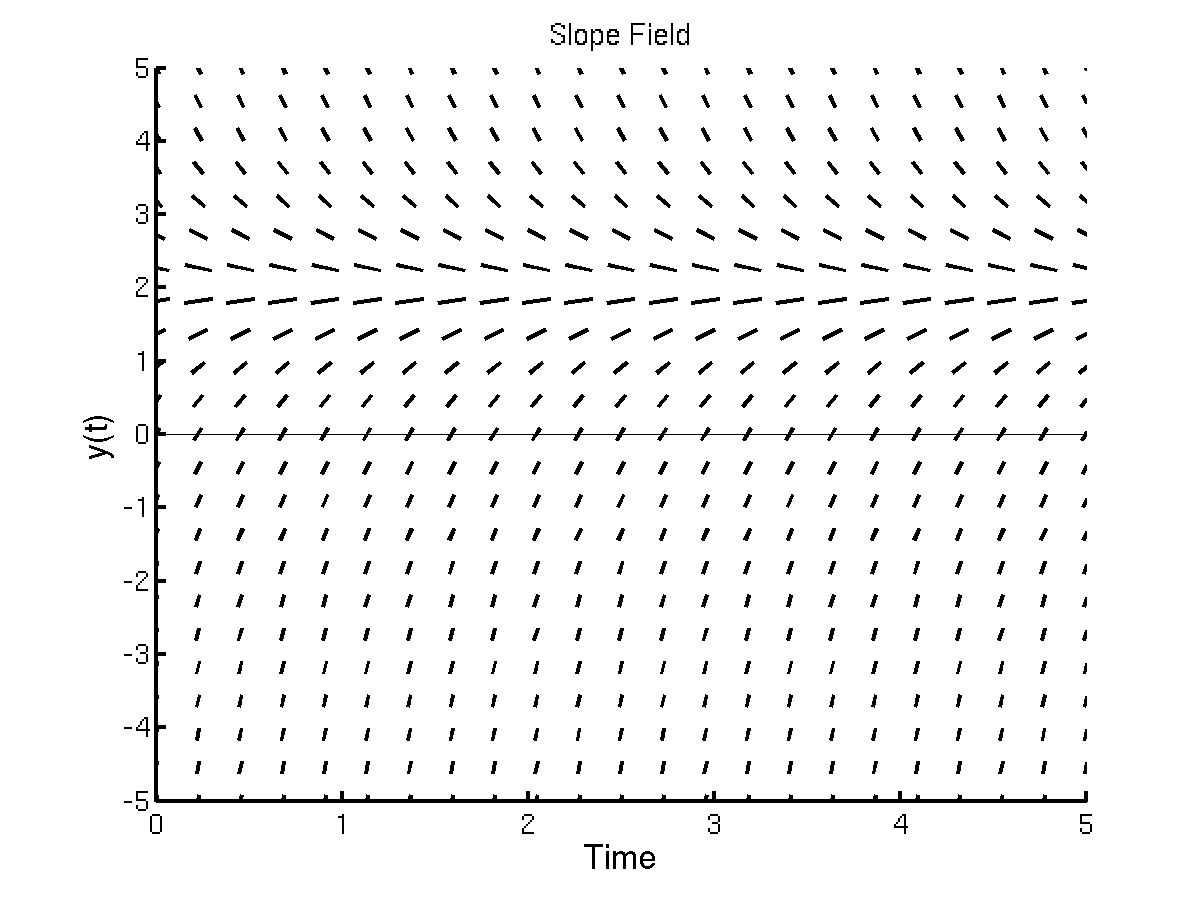
\includegraphics[height=3.0in]{img/sfSteadyWk1}
    \item 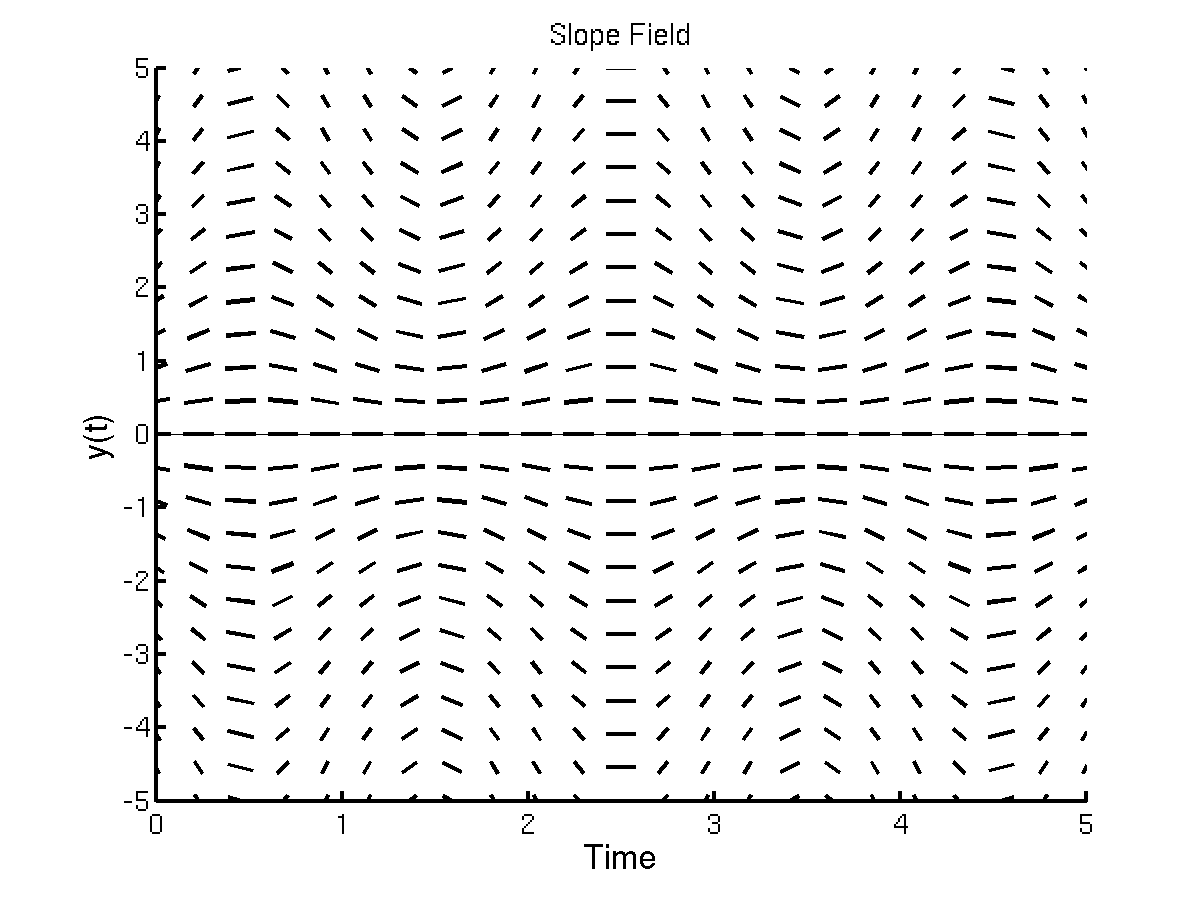
\includegraphics[height=3.0in]{img/sfOscillateWk1}

      \clearpage

    \item 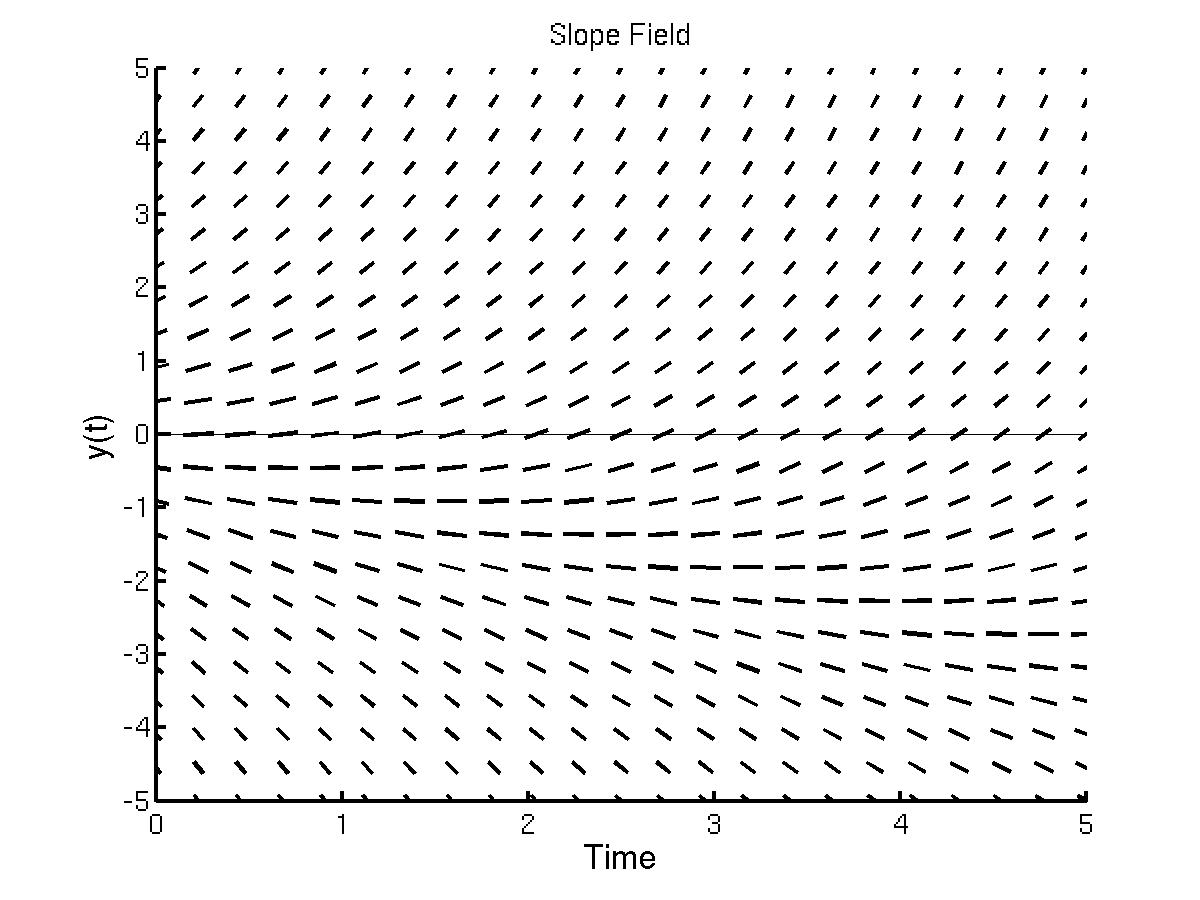
\includegraphics[height=4.0in]{img/sfLinearWk1}
    \item 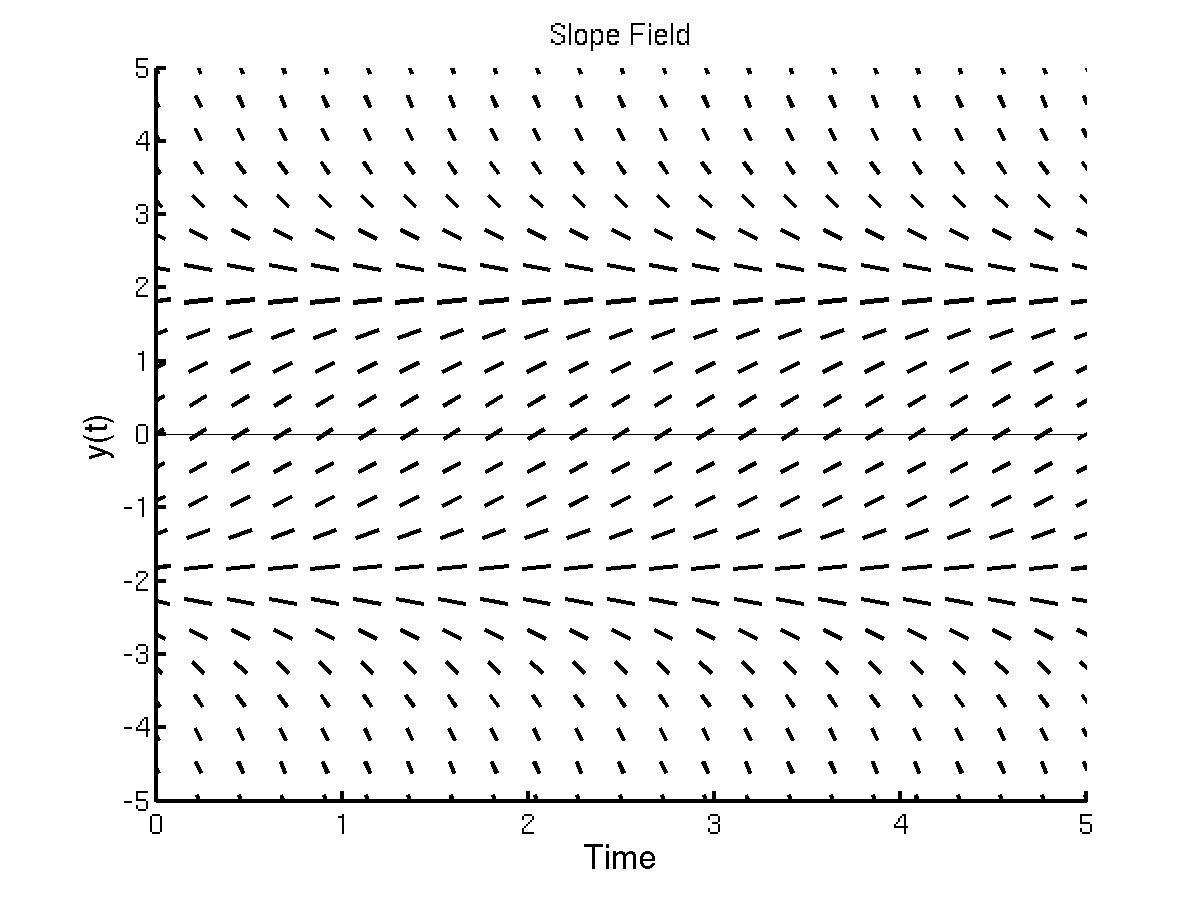
\includegraphics[height=4.0in]{img/sfStabilityWk1}

  \end{subproblem}

\end{problem}


\actTitle{The Chain Rule}
\begin{problem}
  \item Suppose that $3t+C=\ln(y(t))$ where $C$ is a constant. Solve
    the equation for $y(t)$.

    \vfill

  \item The function $y(t)$ depends on $t$. Use the chain rule to find
    the derivative of $\ln(y(t))$.
    \vfill

    \clearpage

  \item Show that the relationship $3t+C=\ln(y(t))$ can also be
    expressed as $y'=3y$.

    \vfill

  \item Show that for any constant $k$ the function
    \begin{eqnarray*}
      y(t) & = & k e^{5t}
    \end{eqnarray*}
    is a solution to the differential equation 
    \begin{eqnarray*}
      y' & = & 5y.
    \end{eqnarray*}
    \vfill

\end{problem}
      % 1

\preClass{Integral Calculus Review}

\begin{problem}
\item Expand each expression using partial fractions. Find the general
  expansion and then solve for the constants.(See the opposite page.)
  \begin{subproblem}
  \item $\frac{y}{y^2-4}$

      \iftoggle{solutions}{%

        \begin{eqnarray*}
          \frac{y}{y^2-4} & = & \frac{y}{(y-2)(y+2)}, \\
          & = &  \frac{A}{y-2} + \frac{B}{y+2}, \\
          & = & \frac{\half}{y-2} + \frac{\half}{y+2}.
        \end{eqnarray*}
        
      }

    \vfill

  \item $\frac{4}{y^2-2y}$.

      \iftoggle{solutions}{%

        \begin{eqnarray*}
          \frac{4}{y^2-2y} & = & \frac{4}{y(y-2)}, \\
          & = & \frac{a}{y} + \frac{b}{y-2}, \\
          & = & \frac{-2}{y} + \frac{2}{y-2}.
        \end{eqnarray*}
        
      }

    \vfill

    \clearpage
      
  \item $\frac{3}{y^2-3y+2}$

      \iftoggle{solutions}{%

        \begin{eqnarray*}
          \frac{3}{y^2-3y+2} & = & \frac{3}{(y-2)(y-1)}, \\
          & = & \frac{a}{y-2} + \frac{b}{y-2}, \\
          & = & \frac{3}{y-2} - \frac{3}{y-1}.
        \end{eqnarray*}
        
      }

    \vfill

  \end{subproblem}
\end{problem}


  \actTitle{Separable ODEs}
  \begin{problem}
  \item Expand each expression using partial fractions and solve for
    the constants:
    \begin{subproblem}
    \item $\frac{3}{y^2-5y-6}$

      \iftoggle{solutions}{%

        \begin{eqnarray*}
          \frac{3}{y^2-5y-6} & = & \frac{a}{y-6} + \frac{b}{y+1}, \\
          & = & \frac{3/7}{y-6} - \frac{3/7}{y+1}.
        \end{eqnarray*}
        
      }

      \vfill

    \item $\frac{-5}{y^3-y^2}$.

      \iftoggle{solutions}{%

        \begin{eqnarray*}
          \frac{-5}{y^3-y^2} & = & \frac{a}{y} + \frac{b}{y^2} + \frac{c}{y-1}, \\
          & = & \frac{5}{y} + \frac{5}{y^2} - \frac{5}{y-1}.
        \end{eqnarray*}
        
      }

      \vfill
      
    \item $\frac{1}{y^3+2y^2+y}$

      \iftoggle{solutions}{%

        \begin{eqnarray*}
          \frac{1}{y^3+2y^2+y} & = & \frac{a}{y} + \frac{b}{y+1} + \frac{c}{(y+1)^2}, \\
          & = & \frac{1}{y} - \frac{1}{y+1} - \frac{1}{(y+1)^2}.
        \end{eqnarray*}
        
      }

      \vfill

    \end{subproblem}

    \clearpage

  \item Find the solutions to the following ODEs. 
    \begin{subproblem}
    \item $y' = y^2 + 1$, $y(0)=3$.

      \iftoggle{solutions}{%

        \begin{eqnarray*}
          y' & = & y^2 + 1, \\
          \frac{y'}{y^2+1} & = & 1, \\
          \int \frac{y'}{y^2+1} ~ dt & = & \int 1 ~ dt, \\
          \arctan(y) & = & t + C, \\
          \arctan(3) & = & C, \\
          y & = & \tan\lp t + \arctan(3)\rp.
        \end{eqnarray*}
        
      }

      \vfill
    \item $y' = yt - t$, $y(0)=4$.

      \iftoggle{solutions}{%

        \begin{eqnarray*}
          y' & = & yt - t, \\
          y' - yt & = & -t, \\
          y' e^{-t^2/2} - e^{-t^2/2} t y & = & - t e^{-t^2/2}, \\
          \frac{d}{dt} \lp y e^{-t^2/2} \rp & = & \int -t e^{-t^2/2} ~ dt, \\
          y e^{-t^2/2} & = & e^{-t^2/2} + C, \\
          4 & = & 1 + C, \\
          C & = & 3, \\
          y & = & 1 + 3e^{t^2/2}.
        \end{eqnarray*}
        
      }

      \vfill

      \clearpage

    \item $y' = 3 \lp y^2 - 5y - 6 \rp$, $y(0)=10$.

      \iftoggle{solutions}{%
        

        See the pre-class activity for the partial fraction expansion.
        \begin{eqnarray*}
          y' & = & 3 \lp y^2 - 5y - 6 \rp, \\
          \frac{y'}{y^2 - 5y - 6} & = & 3, \\
          \int \frac{3/7}{y-6} - \frac{3/7}{y+1} ~ dt & = & \int 3 ~ dt, \\
          \frac{3}{7} \ln(y-6) - \frac{3}{7} \ln(y+1) & = & 3t + C, \\
          \ln\lp\frac{y-6}{y+1}\rp & = & 7t + \frac{7}{3} C, \\
          \frac{y-6}{y+1} & = & k e^{7t}, \\
          \frac{4}{11} & = & k, \\
          \frac{y-6}{y+1} & = & \frac{4}{11} e^{7t}, \\
          y & = & \frac{6+\frac{4}{11} e^{7t}}{1-\frac{4}{11} e^{7t}}.
        \end{eqnarray*}

      }

      \vfill

    \item $y' = y^3 + 2y^2 + y$, $y(0)=5$.

      \iftoggle{solutions}{%
        

        See the pre-class activity for the partial fraction expansion.
        \begin{eqnarray*}
          y' & = & y^3 + 2y^2 + y, \\
          \frac{y'}{y^3 + 2y^2 + y} & = & 1, \\
          \int \frac{1}{y} - \frac{1}{y+1} - \frac{1}{(y+1)^2} ~ dt & = & \int 1 ~ dt, \\
          \ln(y) - \ln(y+1) - \frac{1}{y+1} & = & t + C, \\
          \ln(5) - \ln(6) - \frac{1}{6} & = & C, \\
          \ln(y) - \ln(y+1) - \frac{1}{y+1} & = & t + \ln\lp\frac{5}{6}\rp - \frac{1}{6}.
        \end{eqnarray*}
        the solution is an implicit function of $y(t)$.

      }

      \vfill

    \end{subproblem}

  \end{problem}


  \actTitle{Linear Differential Equations}
  For each problem below $C_1$ and $C_2$ are constants. To show that a
  function is a solution simply substitute it into the left side of
  the equation and then the right. If the results are the same then
  the function is \textbf{a} solution.
  \begin{problem}

  \item Show that $y=C_1 e^{3t}-\frac{1}{3}$ is a solution to the
    differential equation $y'=3y+1$.

      \iftoggle{solutions}{%

        \begin{eqnarray*}
          y' & = & 3 C_1 e^{3t}, \\
          3y + 1 & = & 3C_1 e^{3t} - 1 + 1, \\
                 & = & C_1 e^{3t}.
        \end{eqnarray*}
        
      }

    \vfill

  \item Show that $y=C_1 e^{-t} + C_2 e^{-2t}$ is a solution to the
    differential equation $y''+3y'+2y=0$.

      \iftoggle{solutions}{%

        \begin{eqnarray*}
          y   & = &  C_1 e^{-t} +   C_2 e^{-2t}, \\
          y'  & = & -C_1 e^{-t} - 2 C_2 e^{-2t}, \\
          y'' & = &  C_1 e^{-t} + 4 C_2 e^{-2t}, \\
          C_1 e^{-t} + 4C_2 e^{-2t} - 3C_1 e^{-t} - 6 C_2 e^{-2t} + 2C_1 e^{-t} + 2C_2 e^{-2t} & = & 0.
        \end{eqnarray*}
        
      }

    \vfill

    \clearpage

  \item Suppose that you have the following differential equation:
    \begin{eqnarray}
      \frac{d}{dt} \left( y(t) e^{3t} \right) & = & e^{3t}.
    \end{eqnarray}
    Take the antiderivative of each side and express the result
    without any derivatives. (Do not forget the constant of
    integration.)  

      \iftoggle{solutions}{%

        \begin{eqnarray*}
          y e^{3t} & = & \int e^{3t} ~ dt, \\
          y e^{3t} & = & \frac{1}{3} e^{3t} + C.
        \end{eqnarray*}
        
      }

    
    \vfill

  \item Simplify the expression and solve for $y(t)$. 

      \iftoggle{solutions}{%

        \begin{eqnarray*}
          y & = & \frac{1}{3} + C  e^{-3t}.
        \end{eqnarray*}
        
      }

    \vfill

    \clearpage

  \item Suppose that $y$ is a function of $t$. Use the product rule to
    find the derivative of the function $\left(y(t) e^{3t}\right)$.

      \iftoggle{solutions}{%

        \begin{eqnarray*}
          y' e^{3t} + 3 y e^{3t}
        \end{eqnarray*}
        
      }

    \vfill

  \item Suppose that your final expression in the previous problem is
    equal to $e^{3t}$.  Set that expression equal to $e^{3t}$ and
    simplify as much as possible. What is the new differential
    equation?

      \iftoggle{solutions}{%

        \begin{eqnarray*}
          y' e^{3t} + 3 y e^{3t} & = & e^{3t}, \\
          y' + 3y & = & 1.
        \end{eqnarray*}        
        
      }

      \vfill

  \item What is the solution to the differential equation?

      \iftoggle{solutions}{%

        \begin{eqnarray*}
          y & = & \frac{1}{3} + C e^{-3t}.
        \end{eqnarray*}
        
      }{
        \vspace*{3em}
      }


\end{problem}

        % 2


\preClass{Linear Theory}

\begin{problem}
\item Find the solution to the following differential equation
  \begin{eqnarray}
    \label{eqn:nonhomogeneousPreClass}
    %y' + ty & = & e^{-t}.
    y' + ty & = & t.
  \end{eqnarray}

  \begin{subproblem}
  \item First find a solution to the homogeneous equation
  \begin{eqnarray*}
    y_h' + ty_h & = & 0.
  \end{eqnarray*}

      \iftoggle{solutions}{%

        \begin{eqnarray*}
          y'_h & = & -t y_h, \\
          \frac{y'_h}{y_h} & = & -t, \\
          \ln\lp y_h \rp & = & -\half t^2 + C, \\
          y_h & = & k e^{-t^2/2}.
        \end{eqnarray*}
        
      }

    \vfill

  \item Assume that the solution to equation
    \ref{eqn:nonhomogeneousPreClass} is in the form $y(t) = u(t)
    y_h(t)$ where $y_h(t)$ is your solution to the homogenous
    equation. Take the derivative of $y(t)$. (Use the product rule!)

      \iftoggle{solutions}{%

        \begin{eqnarray*}
          y & = & u \cdot y_h, \\
          y' & = & u' y_h + u y_h'.
        \end{eqnarray*}
        
      }{%

        \vspace*{6em}

      }


    (See the next page.)
    \clearpage

  \item Substitute the function $y(t)$ into the original differential
    equation and solve for $u(t)$. (Do not forget the ``+C'' after
    integrating.)

      \iftoggle{solutions}{%

        \begin{eqnarray*}
          u' y_h + u y_h' + t u y_h & = & t, \\
          u' k e^{-t^2/2} + u (-t) k e^{-t^2/2} + t u k e^{-t^2/2} & = & t, \\
          u' k e^{-t^2/2} & = & t, \\
          u' & = & \frac{1}{k} e^{t^2/2} + C.
        \end{eqnarray*}
        
      }

      \vfill

  \item Substitute the solution, $u(t)$, into your definition,
    $y=u\cdot y_h$, to get the solution to the differential equation.

      \iftoggle{solutions}{%

        \begin{eqnarray*}
          u y_h & = & k e^{-t^2/2} \lp \frac{1}{k} e^{t^2/2} + C \rp, \\
          & = & 1 + \bar{C} e^{-t^2/2}
        \end{eqnarray*}
        
      }{%

        \vspace*{6em}

      }


  \end{subproblem}
\end{problem}


  \actTitle{Growth and Decay}
  \begin{problem}
  \item Sketch a plot of the slope field for the following
    differential equation and make a rough sketch of the solution with
    the given initial condition.
    \begin{eqnarray*}
      A' & = & -0.1 A, \\
      A(0) & = & 1000.
    \end{eqnarray*}
    What is the long term solution? Find the solution to the 
    differential equation. Are your answers consistent?

      \iftoggle{solutions}{%

        \begin{eqnarray*}
          \frac{A'}{A} & = & -0.1, \\
          \ln(A) & = & -.1 t + C, \\
          A & = & k e^{-.1 t}, \\
          A(0) & = & 1000, \\
          1000 & = & k e^0, \\
          A(t) & = & 1000 e^{-.1t}.
        \end{eqnarray*}

        In the long term
        \begin{eqnarray*}
          \lim_{t \rightarrow \infty} A(t) & = & 0.
        \end{eqnarray*}

      }

    \vfill
    \clearpage
  \item The number of bacteria in a colony at 10:00am is approximately
    five million. At noon the number is approximately seven
    million. How many bacteria were in the colony at 9:00am?

    Determine the differential equation. Sketch the slope field, and
    make a prediction based on the sketch. Then determine the solution
    analytically.

      \iftoggle{solutions}{%

        We denote the number of bacteria in the dish at time to be
        $B(t)$. We assume that 10:00am is time zero. The governing
        equation and the solution follow:

        \begin{eqnarray*}
          B' & = & r B, \\
          \Rightarrow B & = & ke^{rt}, \\
          B(0) & = & 5,000,000, \\
          & = & k e^0, \\
          B(t) & = & 5,000,000 e^{rt}, \\
          B(2) & = & 7,000,000, \\
          & = & 5,000,000 e^{2r}, \\
          \frac{7}{5} & = & e^{2r}, \\
          2r & = & \ln(7/5), \\
          r & = & \half \ln(7/5), \\
          B(-1) & = & 5,000,000 e^{-1 \cdot \half \ln(7/5)}, \\
          & \approx & 4,225,771.
        \end{eqnarray*}

      }

    \vfill
  \end{problem}


  \actTitle{Mixing}
  \begin{problem}

  \item A tank initially contains 2,000 litres of water with a
    concentration of mercury of $6.0\times 10^{-5}$ grams per
    litre. Water that contains $3.0\times 10^{-5}$ grams per litre is
    pumped into the tank at 100 litres per hour. The well mixed
    solution is pumped out of the tank at 100 litres per hour.  How
    long will it take for the concentration in the tank to reach
    $4.5\times 10^{-5}$ grams per litre?

    \begin{subproblem}
      \item Draw a picture. Label and define the important quantities.

        \iftoggle{solutions}{%

          \includegraphics[width=20em]{img/tankProblem}

        }{%

          \vfill

        }

      \item Define the quantity to use. Determine the rate that
        mercury moves into the tank, and determine the rate that
        mercury moves out of the tank. Define the initial condition.

        \iftoggle{solutions}{%

          The amount of mercury in the tank at time $t$ is denoted by $A(t)$.

          \begin{eqnarray*}
            \mathrm{rate~in} & = & 3\times10^{-5} \frac{g}{l} \cdot 100 \frac{l}{hr}, \\
            & = & 3\times10^{-3} \frac{g}{hr}.
          \end{eqnarray*}

          \begin{eqnarray*}
            \mathrm{rate~out} & = & A(t) g \cdot \frac{1}{2000~l} \cdot 100 \frac{l}{hr}, \\
            & = & A \cdot \frac{1}{20} \frac{g}{hr}.
          \end{eqnarray*}

          \begin{eqnarray*}
            A(0) & = & 2000~l \cdot 6\times 10^{-5} \frac{g}{l}, \\
            & = & 12\times10^{-2} ~g.
          \end{eqnarray*}

        }

        \vfill

        \clearpage

      \item Write out the differential equation and solve it to find
        the amount of mercury in the tank at any time. Once you find a
        formula for the amount of mercury determine the formula for
        the concentration at any time.

        \iftoggle{solutions}{%

          \begin{eqnarray*}
            A' & = & 3\times10^{-3} - \frac{1}{20} A, \\
            A' + \frac{1}{20} A & = & 3\times10^{-3}, \\
            A' e^{t/20} + \frac{1}{20} e^{t/20} A & = & 3\times10^{-3} e^{t/20}, \\
            \frac{d}{dt} \lp A e^{t/20} \rp & = & 3\times10^{-3} e^{t/20}, \\
            A e^{t/20} & = & 6\times10^{-2 } e^{t/20} + C, \\
            A & = & 6\times10^{-2} + C e^{-t/20}, \\
            A(0) & = & 12\times10^{-2}, \\
            12\times10^{-2} & = & 6\times10^{-2} + C, \\
            C & = & 6\times10^{-2}, \\
            A & = & 6\times10^{-2} + 6\times10^{-2} e^{-t/20}. \\
          \end{eqnarray*}

          The concentration is found by dividing by the volume,
          \begin{eqnarray*}
            \mathrm{Concentration} & = & \frac{6\times10^{-2} + 6\times10^{-2} e^{-t/20}}{2000}.
          \end{eqnarray*}

        }

        \vfill
        

    \end{subproblem}



\end{problem}
   % 3

\chapter{Linear Algebra}


\preClass{Complex Numbers}

\begin{problem}
\item Expand each of the expressions below. (You will need to ``FOIL''
  the expressions.) In each case treat the parameter $i$ as a
  constant number.

  \begin{subproblem}
  \item $(4+3i)*(5-6i)$

      \iftoggle{solutions}{%

        \begin{eqnarray*}
          20 + 15 i - 24 i - 18 i^2 & = & 20 - 9i - 18 i^2.
        \end{eqnarray*}
        
      }

    \vfill

  \item $(2+i)(10+4i)$

      \iftoggle{solutions}{%

        \begin{eqnarray*}
          10 + 10i + 8i + 4i^2 & = & 10 + 18i + 4i^2.
        \end{eqnarray*}
        
      }

    \vfill
      
  \item $(2-i)(2+i)$

      \iftoggle{solutions}{%

        \begin{eqnarray*}
          4 - 2i + 2i  - i^2 & = & 4 - i^2.
        \end{eqnarray*}
        
      }

    \vfill

  \item $(6+3i)(6-3i)$

      \iftoggle{solutions}{%

        \begin{eqnarray*}
          36 + 18i - 18i - 9i^2 & = & 36 - 9 i^2.
        \end{eqnarray*}
        
      }

    \vfill

  \end{subproblem}
\end{problem}



  \actTitle{Complex Numbers}
  \begin{problem}
  \item Find the solution to the following differential equation:
    \begin{eqnarray}
      y' & = & k y, \\
      y(0) & = & 1,
    \end{eqnarray}
    where $k$ is a constant.

    \iftoggle{solutions}{%

      \begin{eqnarray*}
        y(t) & = & C e^{kt}, \\
        y(0) & = & C e^0, \\
        1 & = & C, \\
        y(t) & = & e^{kt}.
      \end{eqnarray*}
        
    }

    \vfill

  \item Replace the constant ``k'' with a constant called ``$i$'' and
    find the solution to the following differential equation:
    \begin{eqnarray}
      y' & = & i y, \\
      y(0) & = & 1.
    \end{eqnarray}
    \label{problem:firstLookEulerFormula}

      \iftoggle{solutions}{%

        \begin{eqnarray*}
          y(t) & = & C e^{it}, \\
          y(0) & = & C e^0, \\
          1 & = & C, \\
          y(t) & = & e^{it}.
        \end{eqnarray*}
        
      }

    \vfill


    \clearpage
  \item Define the constant ``i'' to be $\sqrt{-1}$. Find each of the
    following values:

    \begin{subproblem}
      \item $i^2$

      \iftoggle{solutions}{%

        \begin{eqnarray*}
          i^2 & = & -1.
        \end{eqnarray*}
        
      }

        \vfill
      \item $i^3$

      \iftoggle{solutions}{%

        \begin{eqnarray*}
          i^3 & = & -i.
        \end{eqnarray*}
        
      }

        \vfill
      \item $i*(1+i)$

      \iftoggle{solutions}{%

        \begin{eqnarray*}
          i*(1+i) & = & i + i^2, \\
          & = & i-1.
        \end{eqnarray*}
        
      }

        \vfill
    \end{subproblem}

  \end{problem}


  \actTitle{Complex Numbers}
  \begin{problem}

  \item Define $y(t)$ to be the following function:
    \begin{eqnarray}
      y(t) & = & \cos(t) + i \sin(t).
    \end{eqnarray}
    Answer each of the following questions. Keep in mind that $i$ is a
    constant.

    \begin{subproblem}
      \item Determine the derivative of $y(t)$. 

        \iftoggle{solutions}{%

          \begin{eqnarray*}
            y'(t) & = & -\sin(t) + i \cos(t).
          \end{eqnarray*}
        
        }

        \vfill

      \item Determine and simplify $i*y(t)$.

        \iftoggle{solutions}{%

          \begin{eqnarray*}
            i\cdot y(t) & = & i\cos(t) + i^2 \sin(t), \\
            & = & i\cos(t) - \sin(t).
          \end{eqnarray*}
        
        }

        \vfill

        \clearpage

      \item Show that $y(t)$ is a solution to the following
        differential equation:
        \begin{eqnarray}
          y' & = & i y, \\
          y(0) & = & 1.
        \end{eqnarray}

        \iftoggle{solutions}{%

          \begin{eqnarray*}
            y'(t) & = & -\sin(t) + i \cos(t), \\
            i \cdot y & = & -\sin(t) + i \cos(t), \\
            y(0) & = & \cos(0) + i \sin(0), \\
            & = & 1.
          \end{eqnarray*}
          It is a solution to the differential equation.

        
        }

        \vfill

      \item Recall the solution of the previous differential equation
        given in problem \ref{problem:firstLookEulerFormula}, page
        \pageref{problem:firstLookEulerFormula}. (Write it down here.)

        \iftoggle{solutions}{%

          \begin{eqnarray*}
            y & = & e^{it}.
          \end{eqnarray*}
        
        }{\vspace{4em}}

      \item What is the relationship between that solution and the
        function $y(t)$?

        \iftoggle{solutions}{%

          They are the same.
        
        }

        \vfill
        

    \end{subproblem}

    \clearpage

  \item Express the variable $x$ in terms of $r$ and $\theta$. Do the
    same for $y$. Determine how to find $r$ and $\theta$ given $x$ and
    $y$. 

    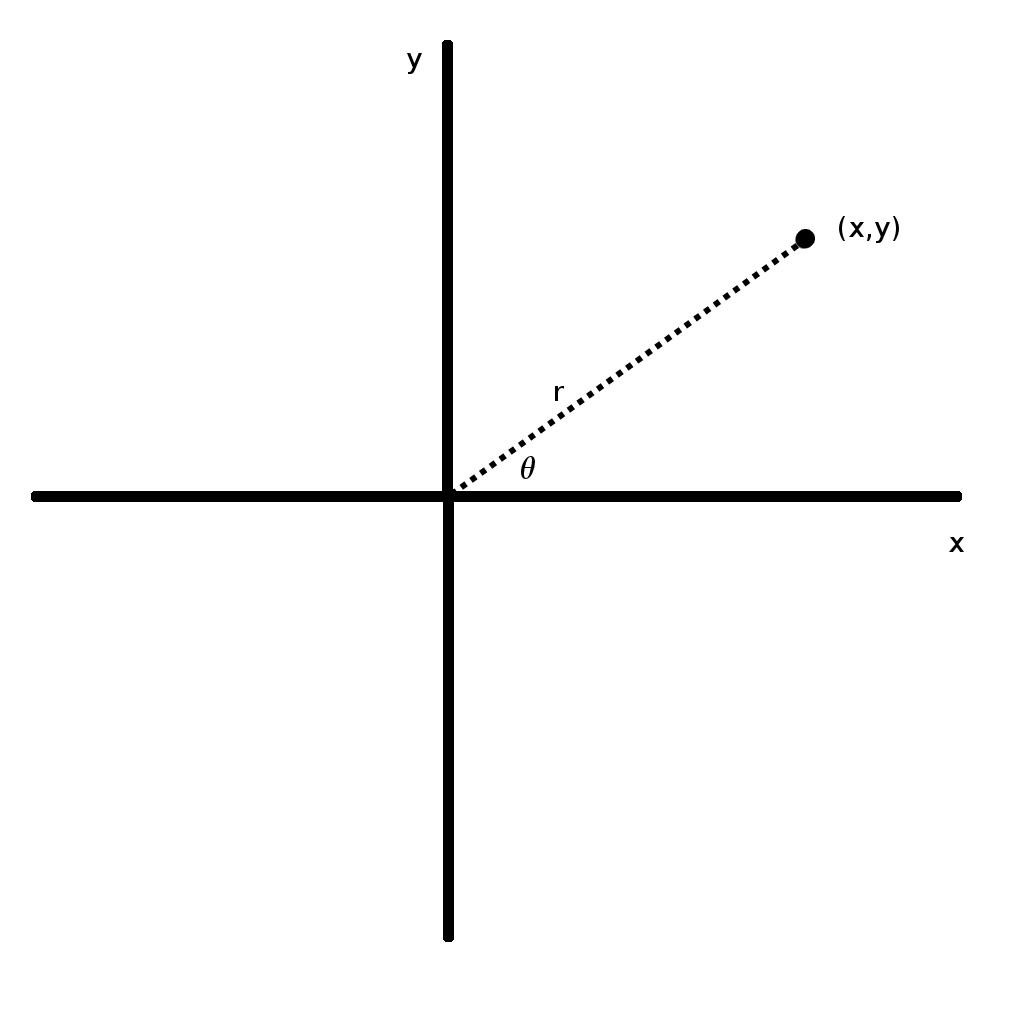
\includegraphics[height=12cm]{img/polar}

    \iftoggle{solutions}{%

      Express $x$ and $y$ in terms of $r$ and $\theta$:
      \begin{eqnarray*}
        x & = & r\cos(\theta), \\
        y & = & r\sin(\theta).
      \end{eqnarray*}

      Express $r$ and $\theta$ in terms of $x$ and $y$:
      \begin{eqnarray*}
        r & = & \sqrt{x^2+y^2}, \\
        \tan(\theta) & = & \frac{y}{x}.
      \end{eqnarray*}
        
    }

    \vfill


  \end{problem}
    % 4

\preClass{Complex Numbers}

\begin{problem}
\item Plot and then convert each point in the complex plane into polar
  coordinates. Label the radius and angle in each case.

  \begin{subproblem}
  \item $3+7i$

      \iftoggle{solutions}{%

        \begin{eqnarray*}
          r & = & \sqrt{3^2 + 7^2}, \\
            & = & \sqrt{58}, \\
          \tan(\theta) & = & \frac{7}{3}, \\
          \theta & \approx & 1.166
        \end{eqnarray*}
        
        \centerline{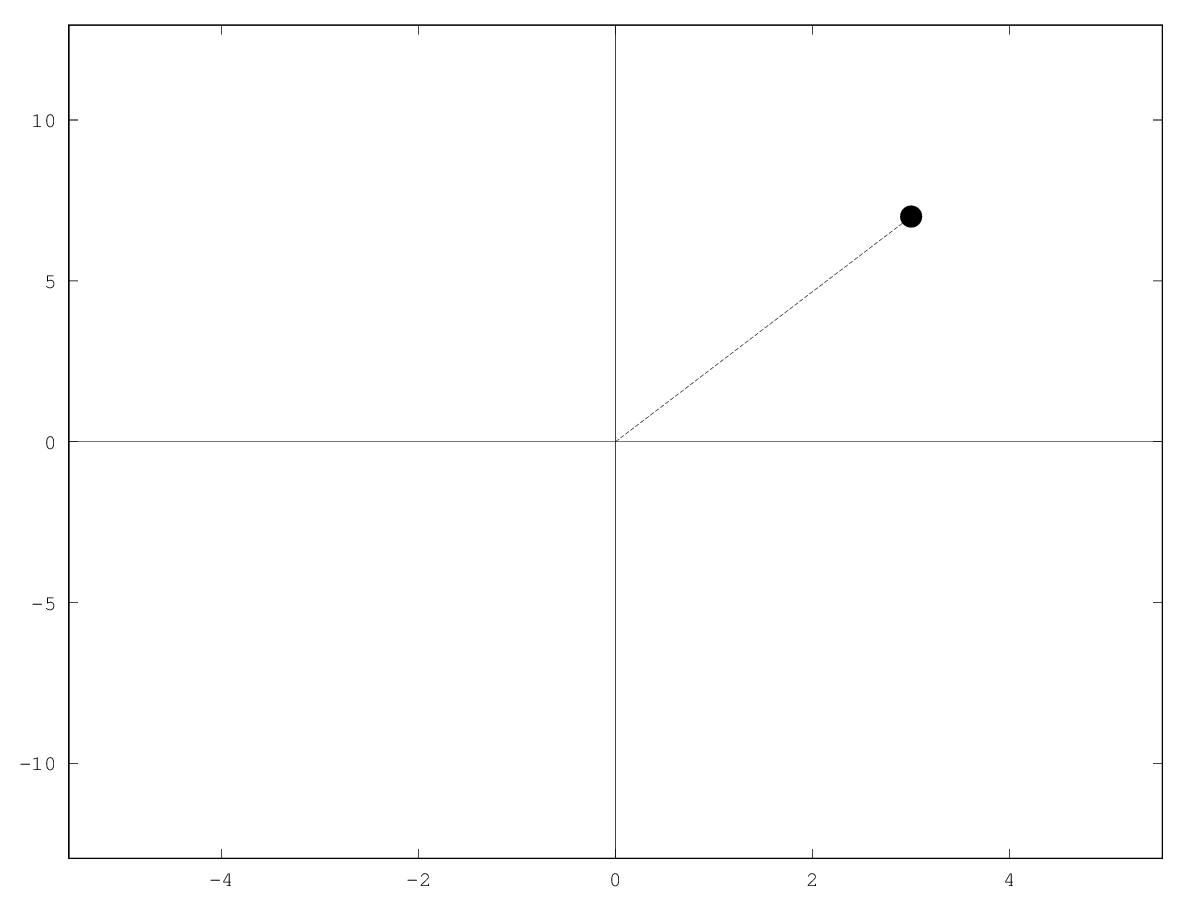
\includegraphics[width=5cm]{img/complexNumber+3+7i}}
      }

    \vfill

  \item $-3+7i$

      \iftoggle{solutions}{%

        \begin{eqnarray*}
          r & = & \sqrt{3^2 + 7^2}, \\
            & = & \sqrt{58}, \\
          \tan(\theta) & = & \frac{7}{-3}, \\
          \theta & \approx & 1.98
        \end{eqnarray*}
        
        \centerline{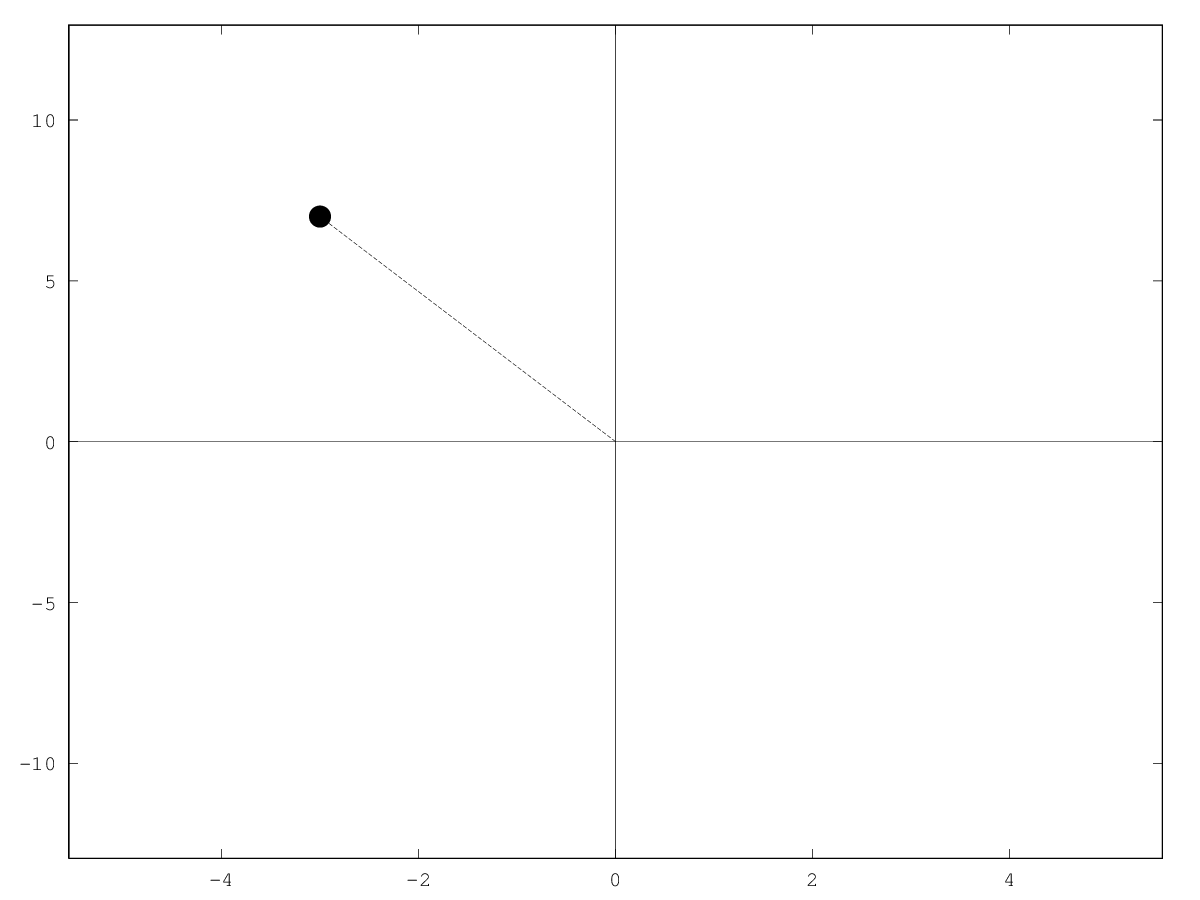
\includegraphics[width=5cm]{img/complexNumber-3+7i}}
        
      }

    \vfill

    (See the next page.)
    \clearpage

  \item $-4+2i$

      \iftoggle{solutions}{%

        \begin{eqnarray*}
          r & = & \sqrt{(-4)^2+2^2}, \\
            & = & \sqrt{20}, \\
          \tan(\theta) & = & \frac{2}{-4}, \\
          \theta & \approx & 2.18
        \end{eqnarray*}
        
        \centerline{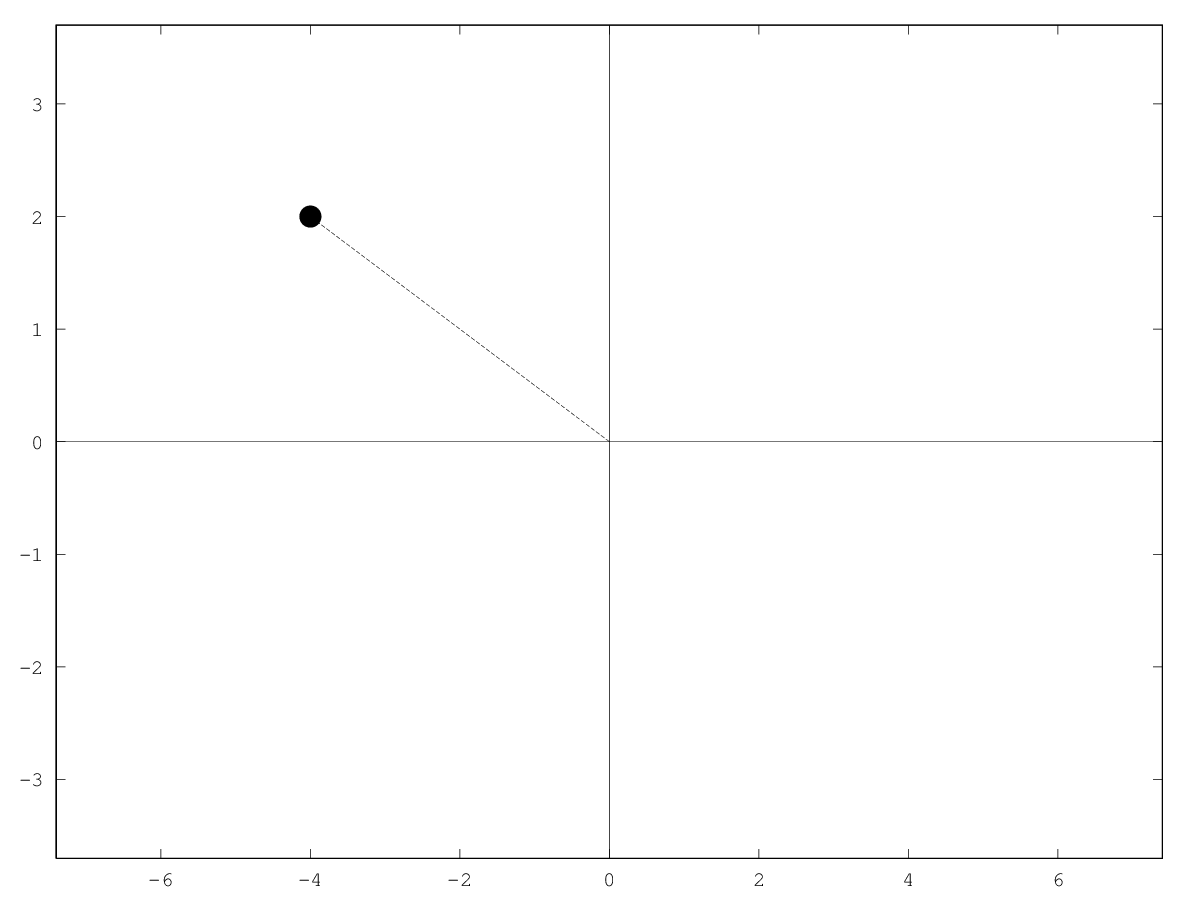
\includegraphics[width=5cm]{img/complexNumber-4+2i}}
        
      }

    \vfill

  \item $3-1i$

      \iftoggle{solutions}{%

        \begin{eqnarray*}
          r & = & \sqrt{3^2+(-1)^2}, \\
            & = & \sqrt{10}, \\
          \tan(\theta) & = & \frac{-1}{3}, \\
          \theta & \approx & -.322
        \end{eqnarray*}
        
        \centerline{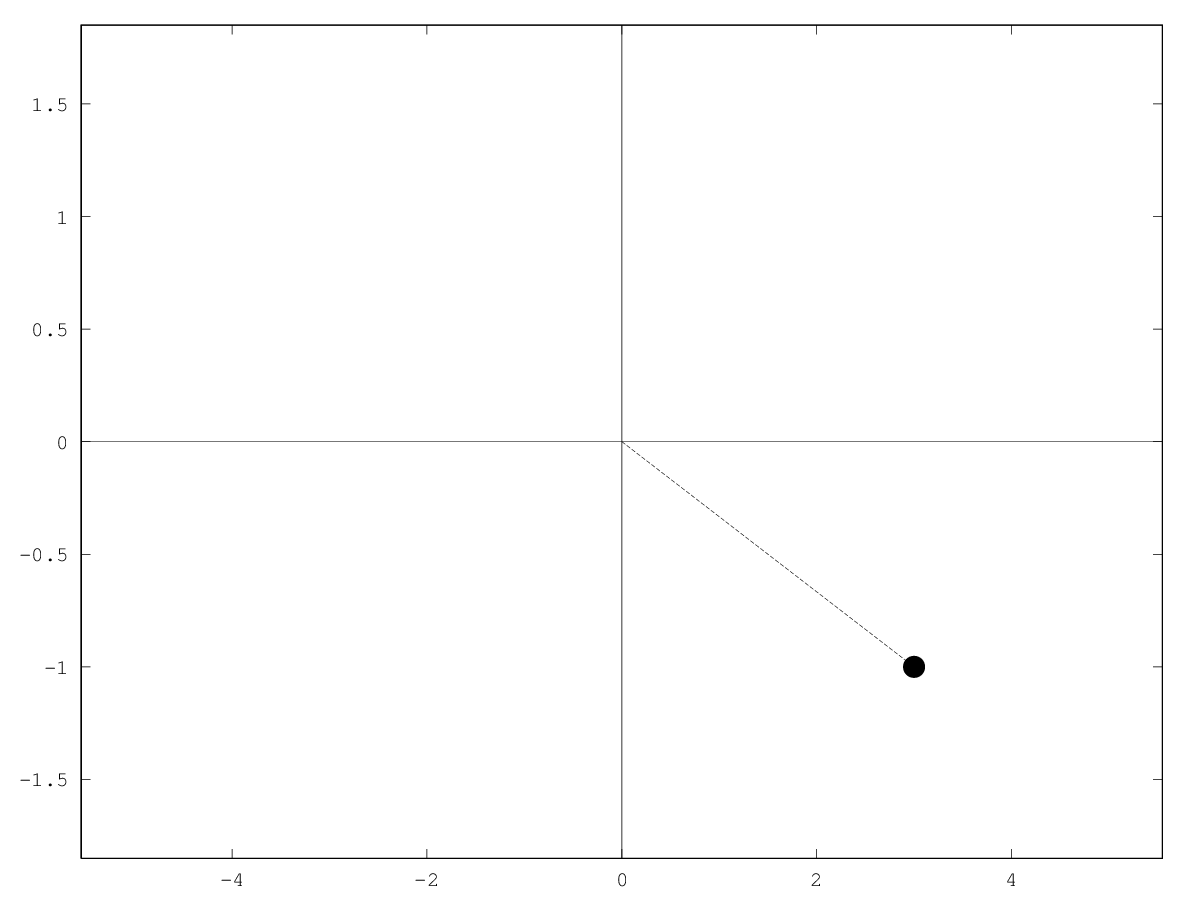
\includegraphics[width=5cm]{img/complexNumber+3-i}}

      }

    \vfill

  \end{subproblem}
\end{problem}


  \actTitle{Complex Numbers}
  \begin{problem}
  \item Expand and simplify the following expressions:
    \begin{subproblem}
      \item $(1+i)(3-i)$

      \iftoggle{solutions}{%

        \begin{eqnarray*}
          (1+i)(3-i)& = & 3 + 3i - i + 1, \\
          & = & 4 + 2i.
        \end{eqnarray*}
        
      }

        \vfill

      \item $(3+2i)(1-i)(7+2i)$

      \iftoggle{solutions}{%

        \begin{eqnarray*}
          (3+2i)(1-i)(7+2i) & = & (3 + 2i - 3i + 2)(7+2i), \\
          & = & (5-i)(7+2i), \\
          & = & 35 + 10i - 7i + 2, \\
          & = & 37 + 3i.
        \end{eqnarray*}
        
      }

        \vfill

      \item $\frac{1+2i}{4+7i}$

      \iftoggle{solutions}{%

        \begin{eqnarray*}
          \frac{1+2i}{4+7i} & = &
          \frac{1+2i}{4+7i}\cdot\frac{4-7i}{4-7i}, \\
          & = & \frac{18 + 15 i}{65}, \\
          & = & \frac{18}{65} + \frac{15}{65} i.
        \end{eqnarray*}
        
      }

        \vfill

      \item $\frac{\overline{4-i}}{3-i}(2+i)$

      \iftoggle{solutions}{%

        \begin{eqnarray*}
          \frac{\overline{4-i}}{3-i}(2+i) & = & \frac{(4+i)(2+i)}{3-i}, \\
          & = & \frac{7+6i}{3-i}, \\
          & = & \frac{7+6i}{3-i}\cdot\frac{3+i}{3+i}, \\
          & = & \frac{15 + 25i}{10}, \\
          & = & \frac{3}{2} + \frac{5}{2}i.
        \end{eqnarray*}
        
      }

        \vfill

    \end{subproblem}

    \clearpage

  \item Express each of the following numbers in the form $a+bi$:
    \begin{subproblem}
    \item $e^{i\pi/4}$

      \iftoggle{solutions}{%

        \begin{eqnarray*}
          e^{i\pi/4} & = & \cos\lp\frac{\pi}{4}\rp + i \sin\lp\frac{\pi}{4}\rp, \\
          & = & \frac{\sqrt{2}}{2} + i \frac{\sqrt{2}}{2}.
        \end{eqnarray*}
        
      }

      \vfill
    \item $2e^{i 3\pi/2}$

      \iftoggle{solutions}{%

        \begin{eqnarray*}
          2e^{i 3\pi/2} & = & 2 \cos\lp\frac{3\pi}{2}\rp + 2\sin\lp\frac{3\pi}{2}\rp, \\
          & = & -2i.
        \end{eqnarray*}
        
      }

      \vfill
    \item $10e^{i \pi/3}$

      \iftoggle{solutions}{%

        \begin{eqnarray*}
          10e^{i \pi/3} & = & 10 \cos\lp\frac{\pi}{3}\rp + i 10 \sin\lp\frac{\pi}{3}\rp, \\
          & = & 5  + i 5\sqrt{3}.
        \end{eqnarray*}
        
      }

      \vfill
    \item $4e^{i \pi}$

      \iftoggle{solutions}{%

        \begin{eqnarray*}
          4e^{i \pi} & = & 4 \cos\lp\pi\rp + i 4 \sin\lp\pi\rp, \\
          &  = & -4.
        \end{eqnarray*}
        
      }

      \vfill
    \end{subproblem}


  \end{problem}


  \actTitle{Complex Numbers}
  \begin{problem}

  \item Plot each of the following numbers in the complex plane and
    then express them in Euler form:
    \begin{subproblem}
      \item $1+i$

      \iftoggle{solutions}{%

        \begin{eqnarray*}
          r & = & \sqrt{1^2 + 1^2}, \\
            & = & \sqrt{2}, \\
          \tan(\theta) & = & \frac{1}{1}, \\
          \theta & = & \frac{\pi}{4}, \\
          z & = & \sqrt{2}e^{i\frac{\pi}{4}}.
        \end{eqnarray*}
        
        \centerline{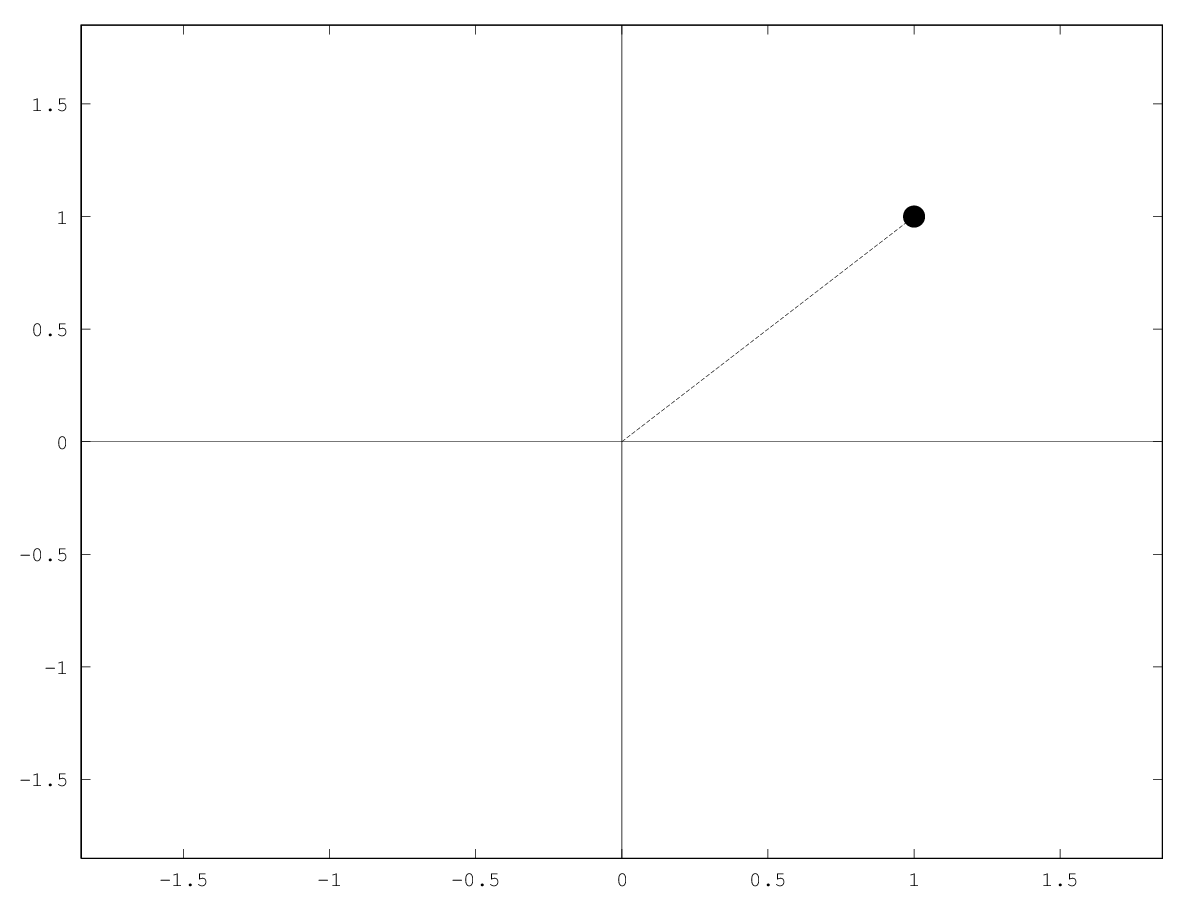
\includegraphics[width=4cm]{img/complexNumber+1+i}}
        
      }

        \vfill
      \item $1-i$

      \iftoggle{solutions}{%

        \begin{eqnarray*}
          r & = & \sqrt{1^2 + (-1)^2}, \\
            & = & \sqrt{2}, \\
          \tan(\theta) & = & \frac{-1}{1}, \\
          \theta & = & \frac{-\pi}{4}, \\
          z & = & \sqrt{2}e^{i\frac{-\pi}{4}}.
        \end{eqnarray*}
        
        \centerline{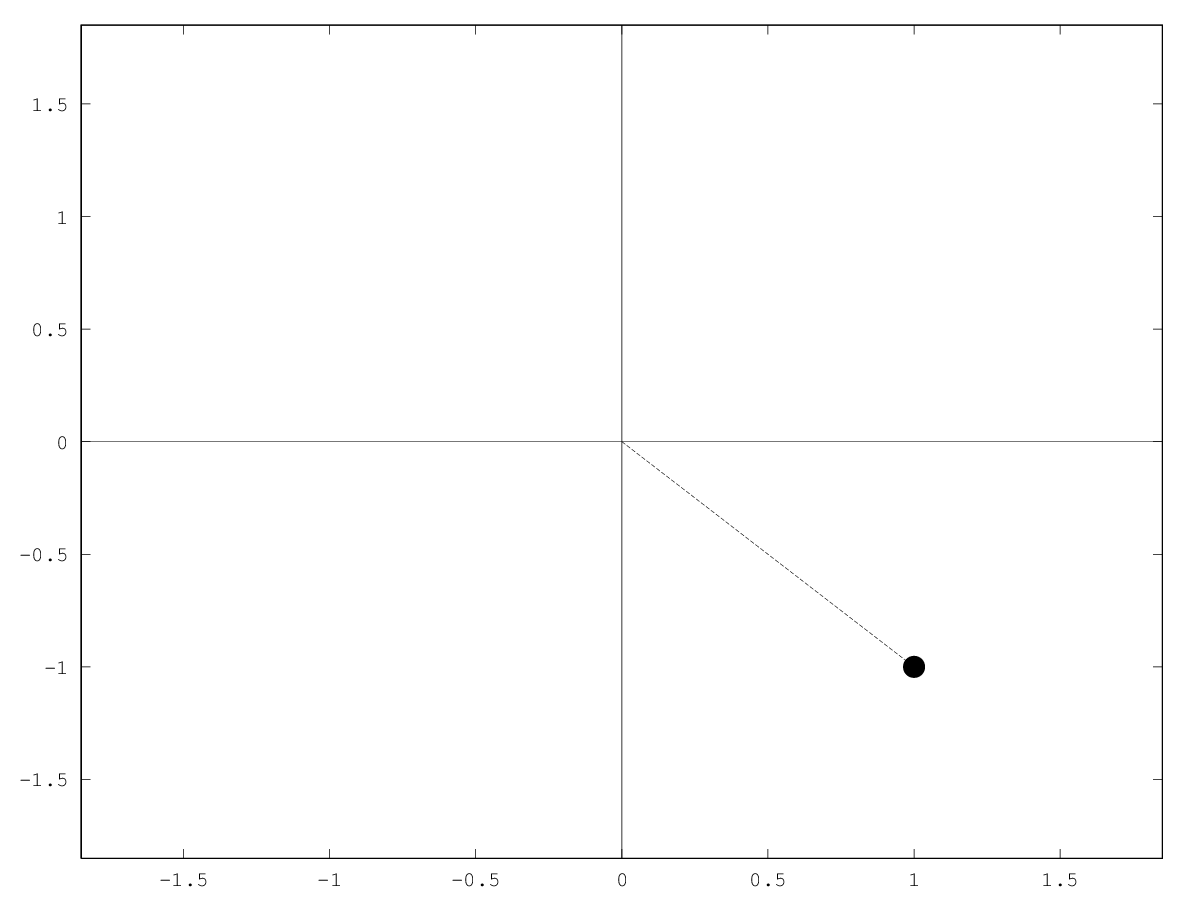
\includegraphics[width=4cm]{img/complexNumber+1-i}}
        
      }

        \vfill
      \item $-1+2i$

      \iftoggle{solutions}{%

        \begin{eqnarray*}
          r & = & \sqrt{(-1)^2 + (2)^2}, \\
            & = & \sqrt{5}, \\
          \tan(\theta) & = & \frac{2}{-1}, \\
          \theta & \approx & 2.03, \\
          z & \approx & \sqrt{5}e^{i2.03}.
        \end{eqnarray*}
        
        \centerline{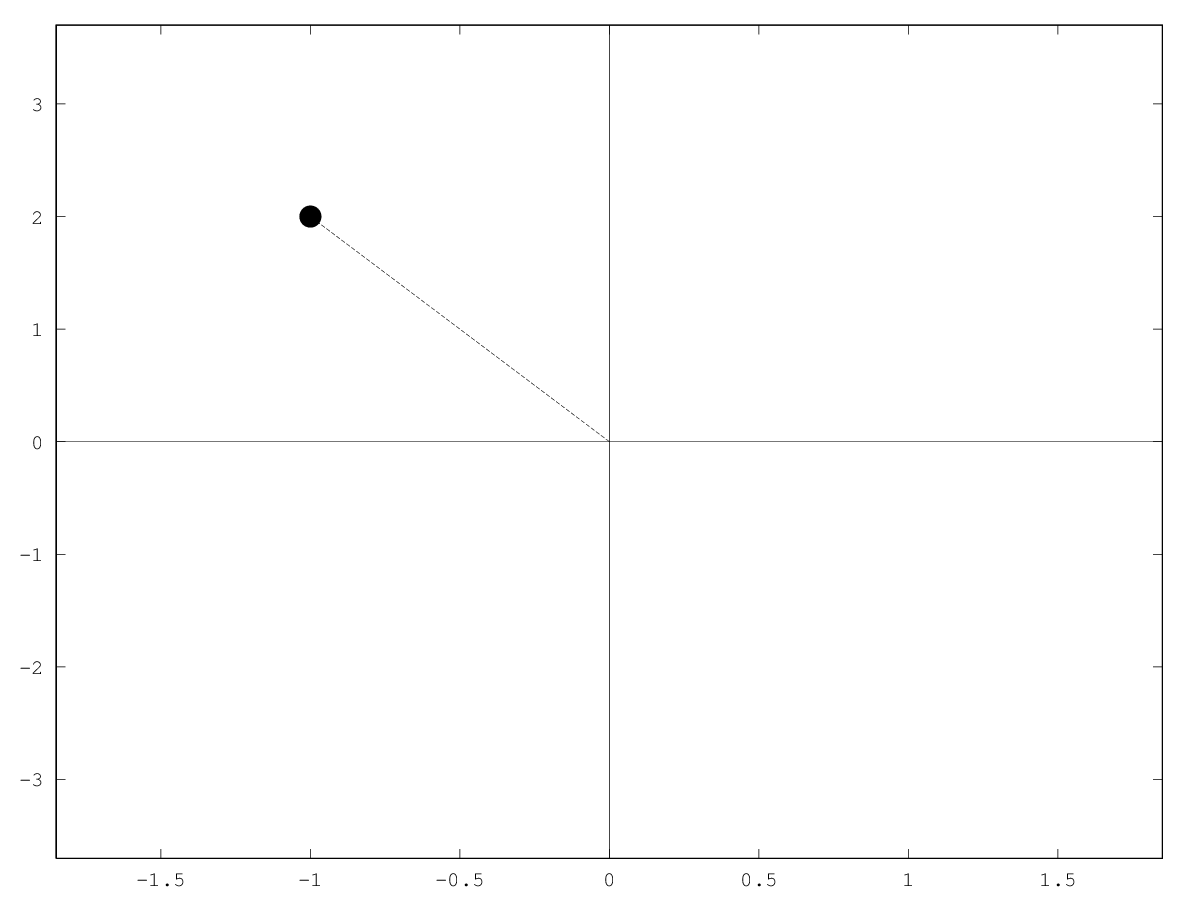
\includegraphics[width=4cm]{img/complexNumber-1+2i}}
        
      }

        \vfill
      \item $-3-i$

      \iftoggle{solutions}{%

        \begin{eqnarray*}
          r & = & \sqrt{(-3)^2 + (-1)^2}, \\
            & = & \sqrt{10}, \\
          \tan(\theta) & = & \frac{-1}{-3}, \\
          \theta & \approx & -2.82, \\
          z & \approx & \sqrt{5}e^{-i2.82}.
        \end{eqnarray*}
        
        \centerline{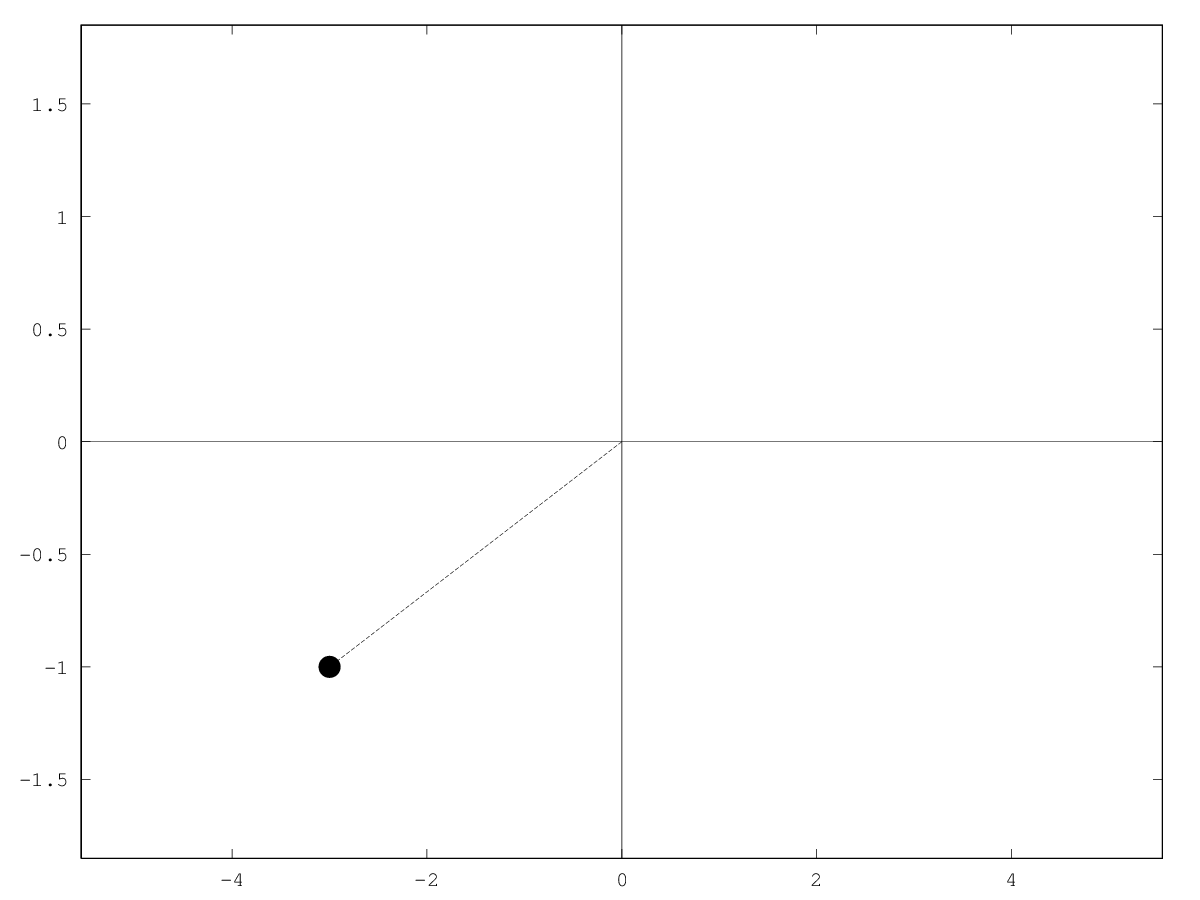
\includegraphics[width=4cm]{img/complexNumber-3-i}}
        
      }

        \vfill
    \end{subproblem}

    \clearpage

  \item Determine the values of the roots. For each problem show the
    graphical representation of the root in relation to the number
    that you are taking the root of.
    \begin{subproblem}
      \item $\sqrt[4]{i}$. 

      \iftoggle{solutions}{%

        \begin{eqnarray*}
          z & = & r e^{i\theta}, \\
          z^4 & = & r^4 e^{i4\theta}, \\
          r^4 e^{i4\theta} & = & e^{i\pi/2},~e^{i5\pi/2},~e^{i9\pi/2},~e^{i13\pi/2}, \\
          z & = & e^{i\pi/8},~e^{i5\pi/8},~e^{i9\pi/8},~e^{i13\pi/8}.
        \end{eqnarray*}
        
      }

        \vfill

      \item $\sqrt[3]{1}$.

      \iftoggle{solutions}{%

        \begin{eqnarray*}
          z & = & r e^{i\theta}, \\
          z^3 & = & r^3 e^{i3\theta}, \\
          r^3 e^{i3\theta} & = & e^{i0},~e^{i2\pi},~e^{i4\pi}, \\
          z & = & 1,~e^{i2\pi/3},~e^{i4\pi/3}.
        \end{eqnarray*}
        
      }

        \vfill

      \item $\sqrt{-4}$.

      \iftoggle{solutions}{%

        \begin{eqnarray*}
          z & = & r e^{i\theta}, \\
          z^2 & = & r^2 e^{i2\theta}, \\
          r^2 e^{i2\theta} & = & e^{i\pi},~e^{i3\pi}, \\
          z & = & e^{i\pi/2},~e^{i3\pi/2}.
        \end{eqnarray*}
        
      }

        \vfill

      \item $\sqrt[5]{1+i}$.

      \iftoggle{solutions}{%

        \begin{eqnarray*}
          z & = & r e^{i\theta}, \\
          z^5 & = & r^5 e^{i5\theta}, \\
          r^5 e^{i5\theta} & = & \sqrt{2}e^{i\pi/4},~\sqrt{2}e^{i9\pi/2},~\sqrt{2}e^{i17\pi/2},~\sqrt{2}e^{i25\pi/2},~\sqrt{2}e^{i33\pi/2}, \\
          z & = & 2^{1/10}e^{i\pi/20},~2^{1/10}e^{i9\pi/20},~2^{1/10}e^{i17\pi/20},~2^{1/10}e^{i25\pi/20},~2^{1/10}e^{i33\pi/20}.
        \end{eqnarray*}
        
      }

        \vfill

    \end{subproblem}

    \clearpage



  \end{problem}
  % 5


\preClass{Linear Algebra}

\begin{problem}
\item Find the solution to the following linear system of equations:
  \begin{eqnarray*}
    3x + 4y & = & 1, \\
    x + y   & = & 0.
  \end{eqnarray*}
  \vfill

\item Find the solution to the following linear system of equations:
  \begin{eqnarray*}
    2x + y & = &  2, \\
    x - y  & = &  1.
  \end{eqnarray*}
  \vfill

\end{problem}


  \actTitle{Linear Algebra}
  \begin{problem}
  \item For the questions below the following matrices are defined:
    \begin{eqnarray*}
      A & = & 
      \left[
        \begin{array}{rr}
          1 &  7 \\ 
          3 & -2
        \end{array}
      \right], \\
      B & = & 
      \left[
        \begin{array}{rr}
          1 &  1 \\
          -1 & -1
        \end{array}
      \right]. \\
    \end{eqnarray*}

    \begin{subproblem}
    \item Determine the value of  $A*B$.

    \vfill

  \item Determine the value of $B*A$.
    \vfill

  \end{subproblem}

    \clearpage
  \item Find the length of the following vectors:

    \begin{subproblem}
      \item $3\vec{\imath} - 2\vec{\jmath} + 2\vec{k}$
        \vfill
      \item $\left[\begin{array}{r} 5 \\ 8 \\ 1 \end{array}\right]$
        \vfill
      \item $<5,-1,3>$
        \vfill
    \end{subproblem}

  \end{problem}


  \actTitle{Linear Algebra}
  \begin{problem}

  \item Find the angles between the following vectors:

    \begin{subproblem}
      \item $3\vec{\imath} - 2\vec{\jmath} + 2\vec{k}$ 
        and $2\vec{\imath} + \vec{\jmath}  + 4\vec{k}$
        \vfill

      \item $\left[\begin{array}{r} 5 \\  8 \\ 1 \end{array}\right]$
        and $\left[\begin{array}{r} 1 \\ -2 \\ 6 \end{array}\right]$
        \vfill

    \end{subproblem}

    \clearpage

  \item Show that the system of equations given by
    \begin{eqnarray*}
      3x + 4y & = & 1, \\
      x + y   & = & 0.
    \end{eqnarray*}
    is equivalent to the system given by
  \begin{eqnarray*}
    \left[
      \begin{array}{rr}
        3 & 4 \\ 
        1 & 1
      \end{array}
    \right] 
    \left[
      \begin{array}{r}
        x \\
        y
      \end{array}
    \right]
    & = & 
    \left[
      \begin{array}{r}
        1 \\
        0
      \end{array}
    \right].
  \end{eqnarray*}


    \vfill

    \clearpage

  \item After finding the requested matrices state what this implies
    about finding the solutions to linear equations.

    \begin{subproblem}
    \item Find a matrix, $A$, so that
      \begin{eqnarray*}
        A * \left[
          \begin{array}{rr}
            3 & 4 \\ 
            1 & 1
          \end{array}
        \right] 
        & = & 
        \left[
          \begin{array}{rr}
             1 & 0 \\ 
             1 & 1
          \end{array}
        \right] 
      \end{eqnarray*}
      
      \vfill

    \item Find a matrix, $B$, so that
      \begin{eqnarray*}
        B * A * \left[
          \begin{array}{rr}
            3 & 4 \\ 
            1 & 1
          \end{array}
        \right] 
        & = & 
        \left[
          \begin{array}{rr}
             1 & 0 \\ 
             0 & 1
          \end{array}
        \right] 
      \end{eqnarray*}

      \vfill

      \end{subproblem}
\end{problem}


     % 6
\part{Matrices}
\lecture{Matrices}{Matrices}
\section{Matrices}

\title{Ordinary Differential Equations}
\subtitle{Math 232 - Matrices}
\date{18 October 2013}

\begin{frame}
  \titlepage
\end{frame}

\begin{frame}
  \frametitle{Outline}
  \tableofcontents[ currentsection ]
\end{frame}


\subsection{Matrix Inverse}


\begin{frame}
  \frametitle{Inverse of a Matrix}

  Suppose that we have the following system:
  \begin{eqnarray*}
    3x + y & = & 4 \\
    2x + y & = & -1
  \end{eqnarray*}

  Another way to express this:
  \begin{eqnarray*}
    \arrayTwo{3}{1}{2}{1} \vecTwo{x}{y} & = & \vecTwo{4}{-1}.
  \end{eqnarray*}

\end{frame}


\begin{frame}
  \frametitle{Interesting Coincidence}

  Note that
  \begin{eqnarray*}
    \arrayTwo{1}{-1}{-2}{3} \arrayTwo{3}{1}{2}{1}  & = & \arrayTwo{1}{0}{0}{1}.
  \end{eqnarray*}

  This means that we can go back to the previous equation to get
  \begin{eqnarray*}
    \arrayTwo{3}{1}{2}{1} \vecTwo{x}{y} & = & \vecTwo{4}{-1}, \\
    \arrayTwo{1}{-1}{-2}{3} \arrayTwo{3}{1}{2}{1} \vecTwo{x}{y} & = & 
          \arrayTwo{1}{-1}{-2}{3}\vecTwo{4}{-1}, \\
    \arrayTwo{1}{0}{0}{1} \vecTwo{x}{y} & = & \vecTwo{5}{-11}, \\
    \vecTwo{x}{y} & = & \vecTwo{5}{-11}.
  \end{eqnarray*}


\end{frame}

\subsection{Notation}

\begin{frame}
  \frametitle{Notation}

  \begin{eqnarray*}
    A & = & \arrayTwo{3}{1}{2}{1} \\
    B & = & \arrayTwo{1}{-1}{-2}{3} 
  \end{eqnarray*}

  Then
  \begin{eqnarray*}
    A\cdot B & = & I_2
  \end{eqnarray*}

\end{frame}


\begin{frame}
  \frametitle{The Inverse}

  \begin{definition}[The Matrix Inverse]
    
    {\color{red}If} two matrices satisfy
    \begin{eqnarray*}
      A\cdot B & = & I
    \end{eqnarray*}
    then $B$ is the \textit{\redText{inverse}} of $A$.

    It is denoted as $\redText{A^{-1}}$.
  \end{definition}


  \uncover<2->{%
    Note most matrices do not have an inverse! If $A^{-1}$ exists then
    we say that $A$ is \textit{invertible}.
  }


\end{frame}

\subsection{Calculating the Inverse}

\begin{frame}
  \frametitle{Calculating the Inverse}

  {\color{red}How do we find $A^{-1}$?}
  \begin{eqnarray*}
    \startRowOpsTwo
    \oneRowOpsTwo{3}{1}{1}{0}
    \oneRowOpsTwo{2}{1}{0}{1}
    \stopRowOps
  \end{eqnarray*}

  {\color{blue}We put thisi $[A | I]$ in RREF.} 
  If we can make the left half look like the
  identity matrix then the right half is the inverse.

\end{frame}


\begin{frame}

  \begin{eqnarray*}
    \stateTwo{1/3 R_1}{~} 
    \startRowOpsTwo
    \oneRowOpsTwo{1}{1/3}{1/3}{0}
    \oneRowOpsTwo{2}{1}{0}{1}
    \stopRowOps \\
    \uncover<2->
    {
      \stateTwo{~}{-2R_1+R_2} 
      \startRowOpsTwo
      \oneRowOpsTwo{1}{1/3}{1/3}{0}
      \oneRowOpsTwo{0}{1/3}{-2/3}{1}
      \stopRowOps \\
    }
    \uncover<3->
    {
      \stateTwo{~}{3R_2} 
      \startRowOpsTwo
      \oneRowOpsTwo{1}{1/3}{1/3}{0}
      \oneRowOpsTwo{0}{1}{-2}{3}
      \stopRowOps 
    }
  \end{eqnarray*}

\end{frame}

\begin{frame}
  \begin{eqnarray*}
      \stateTwo{~}{3R_2} 
      \startRowOpsTwo
      \oneRowOpsTwo{1}{1/3}{1/3}{0}
      \oneRowOpsTwo{0}{1}{-2}{3}
      \stopRowOps \\
    \uncover<2->
    {
      \stateTwo{-1/3R_2+R_1}{~} 
      \startRowOpsTwo
      \oneRowOpsTwo{1}{0}{1}{-1}
      \oneRowOpsTwo{0}{1}{-2}{3}
      \stopRowOps 
    }
  \end{eqnarray*}

  \uncover<3->
  {
    The inverse of the matrix is 
    \begin{eqnarray*}
      A^{-1} & = & \arrayTwo{1}{-1}{-2}{3}
    \end{eqnarray*}
  }

\end{frame}


\begin{frame}
  \frametitle{Example}

  Is the matrix
  \begin{eqnarray*}
    \left[\begin{array}{rrr}
        2 & 4 & 4 \\
        1 & 1 & 2 \\
        0 & -1 & 2
      \end{array}\right]
  \end{eqnarray*}
  invertible?

  \uncover<2->
  {
    \begin{eqnarray*}
      \startRowOpsThree
      \oneRowOpsThree{2}{4}{4}{1}{0}{0}
      \oneRowOpsThree{1}{1}{2}{0}{1}{0}
      \oneRowOpsThree{0}{-1}{2}{0}{0}{1}
      \stopRowOps
    \end{eqnarray*}
  }

\end{frame}



\begin{frame}

    \begin{eqnarray*}
      \startRowOpsThree
      \oneRowOpsThree{2}{4}{4}{1}{0}{0}
      \oneRowOpsThree{1}{1}{2}{0}{1}{0}
      \oneRowOpsThree{0}{-1}{2}{0}{0}{1}
      \stopRowOps \\
      \uncover<2->
      {
        \stateThree{1/2 R_1}{~}{~}
        \startRowOpsThree
        \oneRowOpsThree{1}{2}{2}{1/2}{0}{0}
        \oneRowOpsThree{1}{1}{2}{0}{1}{0}
        \oneRowOpsThree{0}{-1}{2}{0}{0}{1}
        \stopRowOps \\
      }
      \uncover<3->
      {
        \stateThree{~}{-R_1+R_2}{~}
        \startRowOpsThree
        \oneRowOpsThree{1}{2}{2}{1/2}{0}{0}
        \oneRowOpsThree{0}{-1}{0}{-1/2}{1}{0}
        \oneRowOpsThree{0}{-1}{2}{0}{0}{1}
        \stopRowOps 
      }
    \end{eqnarray*}


\end{frame}



\begin{frame}
  \begin{eqnarray*}
    \stateThree{~}{~}{~}
    \startRowOpsThree
    \oneRowOpsThree{1}{2}{2}{1/2}{0}{0}
    \oneRowOpsThree{0}{-1}{0}{-1/2}{1}{0}
    \oneRowOpsThree{0}{-1}{2}{0}{0}{1}
    \stopRowOps \\
    \uncover<2->
    {
      \stateThree{~}{-R_2}{~}
      \startRowOpsThree
      \oneRowOpsThree{1}{2}{2}{1/2}{0}{0}
      \oneRowOpsThree{0}{1}{0}{1/2}{-1}{0}
      \oneRowOpsThree{0}{-1}{2}{0}{0}{1}
      \stopRowOps  \\
    }
    \uncover<3->
    {
      \stateThree{~}{R_2+R_3}{~}
      \startRowOpsThree
      \oneRowOpsThree{1}{2}{2}{1/2}{0}{0}
      \oneRowOpsThree{0}{1}{0}{1/2}{-1}{0}
      \oneRowOpsThree{0}{0}{2}{1/2}{-1}{1}
      \stopRowOps 
    }
  \end{eqnarray*}
\end{frame}




\begin{frame}
  \begin{eqnarray*}
    \stateThree{~}{~}{~}
      \startRowOpsThree
      \oneRowOpsThree{1}{2}{2}{1/2}{0}{0}
      \oneRowOpsThree{0}{1}{0}{1/2}{-1}{0}
      \oneRowOpsThree{0}{0}{2}{1/2}{-1}{1}
      \stopRowOps \\
    \uncover<2->
    {
      \stateThree{~}{~}{1/2 R_3}
      \startRowOpsThree
      \oneRowOpsThree{1}{2}{2}{1/2}{0}{0}
      \oneRowOpsThree{0}{1}{0}{1/2}{-1}{0}
      \oneRowOpsThree{0}{0}{1}{1/4}{-1/2}{1/2}
      \stopRowOps  \\
    }
    \uncover<3->
    {
      \stateThree{-2R_3+R_1}{~}{~}
      \startRowOpsThree
      \oneRowOpsThree{1}{2}{0}{0}{1}{-1}
      \oneRowOpsThree{0}{1}{0}{1/2}{-1}{0}
      \oneRowOpsThree{0}{0}{1}{1/4}{-1/2}{1/2}
      \stopRowOps 
    }
  \end{eqnarray*}
\end{frame}


\begin{frame}
  \begin{eqnarray*}
      \stateThree{~}{~}{~}
      \startRowOpsThree
      \oneRowOpsThree{1}{2}{0}{0}{1}{-1}
      \oneRowOpsThree{0}{1}{0}{1/2}{-1}{0}
      \oneRowOpsThree{0}{0}{1}{1/4}{-1/2}{1/2}
      \stopRowOps \\
    \uncover<2->
    {
      \stateThree{-2R_2+R_1}{~}{~}
      \startRowOpsThree
      \oneRowOpsThree{1}{0}{0}{-1}{3}{-1}
      \oneRowOpsThree{0}{1}{0}{1/2}{-1}{0}
      \oneRowOpsThree{0}{0}{1}{1/4}{-1/2}{1/2}
      \stopRowOps 
    }
  \end{eqnarray*}

  \uncover<3->
  {
    \begin{eqnarray*}
      A^{-1} & =  & \arrayThree{-1}{3}{-1}{1/2}{-1}{0}{1/4}{-1/2}{1/2}
    \end{eqnarray*}
  }
  \uncover<4->
  {
   If you \blueText{cannot} make an identity matrix on the left hand side then the
   matrix is \textbf{\blueText{not}} \textit{invertible}.
  }
\end{frame}

\begin{frame}{Quick Check}

  \begin{eqnarray*}
    \arrayThree{ 2}{4}{ 4}{  1}{ 1}{2}{  0}{  -1}{  2} \cdot 
    \arrayThree{-1}{3}{-1}{1/2}{-1}{0}{1/4}{-1/2}{1/2} & = & 
    \arrayThree{1}{0}{0}{0}{1}{0}{0}{0}{1}
  \end{eqnarray*}
  
\end{frame}

\subsection{Algebraic Properties}

\begin{frame}
  \frametitle{Inverse of the product}

  {\color{red}Theorem:} Suppose that two matrices $A$ and $B$ have
  inverses $A^{-1}$ and $B^{-1}$, respectively.  Then the inverse of
  the product of the two matrices exists and
  {\color{orange}$(AB)^{-1} = B^{-1}A^{-1}$}.\\

  \textit{{\color{blue}Proof.}} Since $A^{-1}$ and $B^{-1}$ exist,  
   \begin{equation*} 
     A \cdot A^{-1} = I, B \cdot B^{-1}  =  I. 
   \end{equation*}
   Then the following product reduces to the identity matrix:
   \begin{eqnarray*}
    \lp B^{-1} A^{-1} \rp \lp A B \rp & = & B^{-1} \lp A^{-1} A \rp B, \\
    & = & B^{-1} I B, \\
    & = & B^{-1} B, \\
    & = & I.
  \end{eqnarray*}

  The inverse of $AB$ is $B^{-1}A^{-1}$.

\end{frame}


\begin{frame}
  \frametitle{Solving Linear Systems}

  Suppose we want to solve a linear system
  \begin{eqnarray*}
    A \vec{x} & = & \vec{b}.
  \end{eqnarray*}

  \textbf{If} $A^{-1}$ exists then 
  \begin{eqnarray*}
    A^{-1} A \vec{x} & = & A^{-1} \vec{b}, \\
    \vec{x} & = & A^{-1} \vec{b}.
  \end{eqnarray*}

  \only<2->{
    Note, we are multiplying by $A^{-1}$ on both sides \blueText{on
      the left} hand side. Be very careful about matrix
    algebra. Multiplying on the left is not the same as multiplying on
    the right!
  }

\end{frame}

\begin{frame}
  \frametitle{Solving Homogeneous Systems}
  {\color{blue}
  Suppose we want to solve a linear system
  \begin{eqnarray*}
    A \vec{x} & = & \vec{0}.
  \end{eqnarray*}
  If $A$ is invertible then the homogeneous solution is the
  zero vector.
  }
  {\color{red}Why?} 
   The homogeneous solution is a solution to the following system:
  \begin{eqnarray*}
    A \vec{x}_h & = & \vec{0}.
  \end{eqnarray*}

  \textbf{If} $A^{-1}$ exists then 
  \begin{eqnarray*}
    A^{-1} A \vec{x}_h & = & A^{-1} \vec{0}, \\
    \vec{x}_h & = & A^{-1} \vec{0}, \\
    & = & \vec{0}.
  \end{eqnarray*}

  \textbf{\color{red}If the inverse exists then the solution is unique.}

\end{frame}





% LocalWords:  Clarkson pausesection hideothersubsections
          % 7

\chapter{Second Order Equations}

\preClass{Second order, constant coefficient equations.}

\begin{problem}
\item The following questions refer to the following differential
  equation:
  \begin{eqnarray*}
    y'' - y' - 12y = 0.
  \end{eqnarray*}

  \begin{subproblem}
  \item Show that $y=e^{4t}$ is a solution.
    \vspace{4cm}
  \item Show that $y=e^{-3t}$ is a solution.
    \vspace{4cm}
  \item Show that $y=C_1 e^{4t} + C_2 e^{-3t}$ is a solution for
    any constants $C_1$ and $C_2$. Will the solution grow or
    decay?

    \vfill

  \end{subproblem}

\end{problem}


  \actTitle{Second Order Equations}
  \begin{problem}

  \item The following questions refer to the following differential
    equation:
    \begin{eqnarray*}
      y'' + 3 y' + 2 y = 0.
    \end{eqnarray*}
    \begin{subproblem}
    \item Assume that the solution is in the form $y=Ae^{rt}$. Find
      the first and second derivatives of this function.
      \vfill

    \item Substitute the previous results into the differential equation.
      \vfill
      
    \item Factor the $Ae^{rt}$ and solve for $r$.
      \vfill

    \item Determine general solution to the differential equation.
      \vfill
    
    \end{subproblem}


 
    \clearpage
  \item Find the solutions to the following differential equation:
    \begin{eqnarray*}
      y'' + 3y' - 10y = 0.
    \end{eqnarray*}
    Determine if the solution will exhibit growth or decay. Can you
    determine the answer to the question of stability by only looking
    at the roots of the characteristic equation? If so how?

    \vfill
  \end{problem}


  \actTitle{Second Order Equations}
  \begin{problem}

  \item The questions refer to the following differential equation:
    \begin{eqnarray*}
      y'' + 4y & = & 0.
    \end{eqnarray*}

    \begin{subproblem}
      \item Show that $y=C_1 e^{i2t} + C_2 e^{-i2t}$ is a solution to
        the differential equation.
        \vfill

      \item Use Euler's formula to write the solution, $y=C_1 e^{i2t}
        + C_2 e^{-i2t}$, in terms of sines and cosines.
        \vfill

        \clearpage

      \item Simplify the terms so that the sine and cosine terms are
        only expressed in terms of $\sin(2t)$ and $\cos(2t)$.

        \vfill

      \item Collect all the sine terms and the cosine terms so that
        the solution is in the form
        \begin{eqnarray*}
          y & = & \#_1 \cos(2t) + \#_2 \sin(2t).
        \end{eqnarray*}
        \vfill

      \item Show that $y=k_1 \cos(2t) + k_2 \sin(2t)$ is a solution to
        the original differential equation.
        \vfill
        

    \end{subproblem}


\end{problem}
       %8


\preClass{Second order, constant coefficient equations.}

  \begin{problem}

  \item A spring mass system is constructed. The mass is 0.1 kg. The
    spring is stretched 0.04 m when the mass is hung vertically from
    the spring. The force due to air friction is estimated to be 0.03
    N when the object is moving at 0.2 m/sec. The system is placed in
    a horizontal orientation, and the object is pulled so that the
    spring extends 0.03 m and released from rest.

    \begin{subproblem}
      \item Determine the governing equation for the system. (This
        includes the initial conditions.)
        \vfill

      \item Determine the \textit{general} solution to the differential
        equation. (Do not consider the initial conditions yet.)
        \vfill

        \clearpage

      \item Determine the specific solution to match the initial conditions.

        \vfill

      \item Determine a different value for the spring constant so
        that the system will oscillate with a period of 1.2 seconds.
        \vfill

    \end{subproblem}



  \end{problem}


\actTitle{Second order, linear differential equations}

\begin{problem}
\item A spring mass system is constructed. The mass is $m$ kg. The
  spring is stretched 0.04 m when the mass is hung vertically from the
  spring. The air friction coefficient is $b$.

    \begin{subproblem}
      \item Determine the governing equation for the system. 
        \vfill

      \item Determine the characteristic equation for the differential
        equation. (Do not consider the initial conditions yet.)
        \vfill

        \clearpage

      \item Assume that the solution to the characteristic equation
        will be a complex number so that the system will
        oscillate. Break the solutions into two pieces, the real and
        the imaginary parts.

        \vfill

      \item Find and solve the system of equations that result for $m$
        and $b$ if you wish the amplitude of the system to decay like
        $e^{-t/10}$ and the system to oscillate with a period of 3.1
        seconds.

        \vfill

    \end{subproblem}


\end{problem}


\actTitle{Method of Undetermined Coefficients}

  \begin{problem}
  \item Find the solution to the following differential equation:
    \begin{eqnarray*}
      y'' - 2y' - 8y & = & 3t + 4.
    \end{eqnarray*}
    \begin{subproblem}
    \item Write out the homogeneous equation.
      \vspace{2em}
    \item Find the solution to the homogeneous equation.
      \vfill

    \clearpage

  \item Write out the general form of the particular solution:
    \vspace{2em}

  \item Substitute your particular solution into the non-homogeneous equation.
    \vfill

  \item Solve for the constants.
    \vfill

  \end{subproblem}

  \end{problem}

 %9

\chapter{Systems of Differential Equations}
\part{Eigen-Vectors/Values}
\lecture{EigenVectors/Values}{Eigen-Vectors/Values}
\section{Eigenvalues and Eigenvectors}


\title{Ordinary Differential Equations}
\subtitle{Math 232 - Eigenvalues and eigenvectors}
\date{30 October 2013}

\begin{frame}
  \titlepage
\end{frame}

\begin{frame}
  \frametitle{Outline}
  \tableofcontents[currentsection]
\end{frame}


\subsection{Eigenvalues and Eigenvectors}


\begin{frame}
  \frametitle{Eigenvalues and Eigenvectors}

  Suppose that we have a system of differential equations,
  \begin{eqnarray*}
    \frac{d}{dt} \vec{x} & = & A \vec{x}.
  \end{eqnarray*}
  Assume that $A$ is a square matrix.

  What if we can find a vector, $\vec{v}$, that satisfies
  \begin{eqnarray*}
    A \vec{v} & = & \lambda \vec{v},
  \end{eqnarray*}
  where $\lambda$ is a scalar (number)?

\end{frame}


\begin{frame}
  If so. then....
  \begin{eqnarray*}
    \frac{d}{dt} \vec{v} & = & A \vec{v}, \\
    & = & \lambda \vec{v}.
  \end{eqnarray*}

  \only<1>%
  {
    But,
    \begin{eqnarray*}
      \vec{v} & = & 
      \left[
        \begin{array}{r}
          x_1 \\ x_2 \\ x_3 \\ \vdots \\ x_n
        \end{array}
      \right].
    \end{eqnarray*}
  }
  
  \only<2>%
  {
    This implies that
    \begin{eqnarray*}
      \deriv{x_1}{t} & = & \lambda x_1, \\
      \deriv{x_2}{t} & = & \lambda x_2, \\
      \deriv{x_3}{t} & = & \lambda x_3, \\
      \vdots         &   & \vdots \\
      \deriv{x_n}{t} & = & \lambda x_n
    \end{eqnarray*}

    We can solve each one of these equations separately!
  }

\end{frame}


\begin{frame}
  \frametitle{Eigenvalues and Eigenvectors}

  \begin{definition}
    Given a square matrix, $A$, an \blueText{eigenvector}, $\vec{v}$,
    and an associated \blueText{eigenvalue}, $\lambda$, satisfy
    \begin{eqnarray*}
      A \vec{v} & = & \lambda \vec{v}.
    \end{eqnarray*}
  \end{definition}



\end{frame}


\iftoggle{clicker}{%
\begin{frame}
  \frametitle{Clicker Quiz}

      \ifnum\value{clickerQuiz}=1{%
        We want to solve a system of linear equations
        \begin{eqnarray*}
          A \vec{x} & = & \vec{b}.
        \end{eqnarray*}
        We find the determinant of the matrix $A$, and the determinant is zero. 

        What does this imply about the solutions to the linear system.
        \vfill

        \begin{tabular}{ll}
          A: & The solution is unique. \\
          B: & There are infinite solutions. \\
          C: & There are no solutions. \\
          D: & Either B or C. \\
        \end{tabular}
        \vfill

      }\fi

      \ifnum\value{clickerQuiz}=2{%
        We want to solve a system of linear equations
        \begin{eqnarray*}
          A \vec{x} & = & \vec{b}.
        \end{eqnarray*}
        We find the determinant of the matrix $A$, and the determinant is zero. 

        What does this imply about the solutions to the linear system.
        \vfill

        \begin{tabular}{ll}
          A: & The solution is unique. \\
          B: & There are infinite solutions. \\
          C: & There are no solutions. \\
          D: & Either B or C. \\
        \end{tabular}

        \vfill

     }\fi
   
     \ifnum\value{clickerQuiz}=3{%
        \vfill
        We want to solve a system of linear equations
        \begin{eqnarray*}
          A \vec{x} & = & \vec{b}.
        \end{eqnarray*}
        We find the determinant of the matrix $A$, and the determinant is zero.

        What does this imply about the solutions to the linear system.
        \vfill

        \begin{tabular}{ll}
          A: & The solution is unique. \\
          B: & There are infinitely many solutions. \\
          C: & There are no solutions. \\
          D: & Either B or C. \\
        \end{tabular}

    }\fi
  

\end{frame}
}



\begin{frame}
  \frametitle{How to find}

  Given $A$ how can we find its eigenvalues and eigenvectors?
  \begin{eqnarray*}
    A \vec{v} & = & \lambda \vec{v}, \\
    A \vec{v} - \lambda \vec{v} & = & 0, \\
    A \vec{v} - \lambda \redText{I} \vec{v} & = & 0, \\
    \lp A - \lambda I \rp \vec{v} & = & 0.
  \end{eqnarray*}

  \only<1>{\textit{Remember $\vec{v}$ is a vector and $A$ is an array. We cannot
    add them!}}

  \uncover<2->{\redText{One solution is $\vec{v}=\vec{0}$.}} 
  \uncover<3->{\blueText{We do not like this solution.}}
  \uncover<4->{We must have a situation where there is not a unique solution. If there
    is not a unique solution then this implies that
  \begin{eqnarray*}
    \det\lp A - \lambda I \rp & = & 0.
  \end{eqnarray*}
  Find a value for $\lambda$ that makes this true. (\redText{Note that there
  will be infinitely many solutions for $\vec{v}$.})}

\end{frame}


\begin{frame}
  \frametitle{Finding Eigenvalues and Eigenvectors}

  Given a square matrix, $A$, to find the eigenvalues and eigenvectors do the following:
  \begin{enumerate}
  \item Determine the characteristic equation:
    \begin{eqnarray*}
      \det\lp A - \lambda I \rp & = & 0.
    \end{eqnarray*}
  \item Solve the equation for the \blueText{values} of $\lambda$,
    call them $\lambda_j$.
  \item Find the eigenvector associated with each value of $\lambda_j$,
    \begin{eqnarray*}
      \lp A - \lambda_j I \rp \vec{v}_j & = & \vec{0}.
    \end{eqnarray*}
    (Note that there will be infinitely many solutions for each
    $\vec{v}_j$.) Solving linear systems means dealing with
    RREF. Woohoo!!
  \end{enumerate}

\end{frame}

\subsection{Examples}

\begin{frame}
  \frametitle{Example}

  \begin{eqnarray*}
    A & = & \arrayTwo{12}{-10}{15}{-13}.
  \end{eqnarray*}

  \uncover<2->
  {
    Find the characteristic equation:
    \begin{eqnarray*}
      \det\lp\arrayTwo{12-\lambda}{-10}{15}{-13-\lambda}\rp & = & \lambda^2+\lambda-6.
    \end{eqnarray*}

    Find the values of $\lambda$:
    \begin{eqnarray*}
      \lambda^2+\lambda-6 & = & (\lambda-2)(\lambda+3), \\
      & = & 0.
    \end{eqnarray*}
    So \redText{$\lambda_1 = 2$} and \redText{$\lambda_2=-3$}.
  }

\end{frame}


\begin{frame}
  Find the vectors:

  $\lambda_1 = 2$:
  \begin{eqnarray*}
    \arrayTwo{10}{-10}{15}{-15} \vecTwo{x}{y} & = & \vecTwo{0}{0}, \\
    10x - 10y & = & 0, \\
    15x - 15y & = & 0, \\
    x & = & y.
  \end{eqnarray*}

  The first eigenvector is 
  \begin{eqnarray*}
    \vec{v}_1 & = & \vecTwo{y}{y}, \\
    & = & y \vecTwo{1}{1}.
  \end{eqnarray*}

  \redText{Let}
  \begin{eqnarray*}
    \redText{\vec{v}_1} & \redText{=} & \redText{\vecTwo{1}{1}}.
  \end{eqnarray*}

\end{frame}

\begin{frame}
  Find the vectors:

  $\lambda_2 = -3$:
  \begin{eqnarray*}
    \arrayTwo{15}{-10}{15}{-10} \vecTwo{x}{y} & = & \vecTwo{0}{0}, \\
    15x - 10y & = & 0, \\
    15x - 10y & = & 0, \\
    x & = & \frac{2}{3} y.
  \end{eqnarray*}

  The second eigenvector is 
  \begin{eqnarray*}
    \vec{v}_2 & = & \vecTwo{\frac{2}{3}y}{y}, \\
    & = & y \vecTwo{\frac{2}{3}}{1}.
  \end{eqnarray*}

  \redText{Let}
  \begin{eqnarray*}
    \redText{\vec{v}_2} & \redText{=} & \redText{\vecTwo{2}{3}}.
  \end{eqnarray*}

\end{frame}






\begin{frame}
  \frametitle{Example}

  \begin{eqnarray*}
    A & = & \arrayTwo{4}{18}{-3}{-11}.
  \end{eqnarray*}

  \uncover<2->
  {
    Find the characteristic equation:
    \begin{eqnarray*}
      \det\lp\arrayTwo{4-\lambda}{18}{-3}{-11-\lambda}\rp & = & \lambda^2+7\lambda+10.
    \end{eqnarray*}
    
    Find the values of $\lambda$:
    \begin{eqnarray*}
      \lambda^2+7\lambda+10 & = & (\lambda+2)(\lambda+5), \\
      & = & 0.
    \end{eqnarray*}
    So \redText{$\lambda_1 = -2$} and \redText{$\lambda_2=-5$}.
  }

\end{frame}


\begin{frame}
  Find the vectors:

  $\lambda_1 = -2$:
  \begin{eqnarray*}
    \arrayTwo{6}{18}{-3}{-9} \vecTwo{x}{y} & = & \vecTwo{0}{0}, \\
    6x + 18y & = & 0, \\
    -3x - 9y & = & 0, \\
    x & = & -3y.
  \end{eqnarray*}

  The first eigenvector is 
  \begin{eqnarray*}
    \vec{v}_1 & = & \vecTwo{-3y}{y}, \\
    & = & y \vecTwo{-3}{1}.
  \end{eqnarray*}

  \redText{Let}
  \begin{eqnarray*}
    \redText{\vec{v}_1} & \redText{=} & \redText{\vecTwo{-3}{1}}.
  \end{eqnarray*}

\end{frame}

\begin{frame}
  Find the vectors:

  $\lambda_2 = -5$:
  \begin{eqnarray*}
    \arrayTwo{9}{18}{-3}{-6} \vecTwo{x}{y} & = & \vecTwo{0}{0}, \\
    9x + 18y & = & 0, \\
    -3x - 6y & = & 0, \\
    x & = & -2 y.
  \end{eqnarray*}

  The second eigenvector is 
  \begin{eqnarray*}
    \vec{v}_2 & = & \vecTwo{-2y}{y}, \\
    & = & y \vecTwo{-2}{1}.
  \end{eqnarray*}

  \redText{Let}
  \begin{eqnarray*}
    \redText{\vec{v}_2} & \redText{=} & \redText{\vecTwo{-2}{1}}.
  \end{eqnarray*}

\end{frame}



\begin{frame}
  \frametitle{Theorem - Distinct Eigenvalues Makes Life Easier}

  \begin{theorem}
    If the eigenvalues of an $n\times n$ matrix include \blueText{\textbf{$n$}}
    \blueText{distinct} values then the eigenvectors are linearly
    independent.
  \end{theorem}


  \vfill

  \uncover<2->
  {
    So what? When we start solving DEs it will mean we are essentially
    done. 
  }

  \vfill

\end{frame}



\begin{frame}
  \frametitle{Example}

  See example 5 on page 318.
  \begin{eqnarray*}
    A & = & \arrayThree{-2}{1}{1}{1}{-2}{1}{1}{1}{-2}.
  \end{eqnarray*}

  \uncover<2->
  {
    Find the characteristic equation:
    \begin{eqnarray*}
      \det\lp\arrayThree{-2-\lambda}{1}{1}{1}{-2-\lambda}{1}{1}{1}{-2-\lambda}\rp
      & = & \lambda (\lambda+3)^2.
    \end{eqnarray*}

    Find the values of $\lambda$:
    \begin{eqnarray*}
      \lambda (\lambda+3)^2 & = & 0.
    \end{eqnarray*}
    So \redText{$\lambda_1 = 0$} and \redText{$\lambda_2=-3$}.
  }

\end{frame}



\begin{frame}
  Find the vectors:

  $\lambda_1 = 0$:
  \begin{eqnarray*}
    \arrayThree{-2}{1}{1}{1}{-2}{1}{1}{1}{-2}\vecThree{x}{y}{z} & = & \vecThree{0}{0}{0}, \\
  \end{eqnarray*}

  Express this system in an augmented matrix and put it in reduced row
  echelon form:
  \begin{eqnarray*}
    \mathrm{RREF}\startRowFour
    \oneRowFour{-2}{1}{1}{0} 
    \oneRowFour{1}{-2}{1}{0}
    \oneRowFour{1}{1}{-2}{0}
    \stopRowOps
    & = & 
    \startRowFour
    \oneRowFour{1}{0}{-1}{0} 
    \oneRowFour{0}{1}{-1}{0}
    \oneRowFour{0}{0}{0}{0}
    \stopRowOps
  \end{eqnarray*}


\end{frame}

\begin{frame}
  The first eigenvector is 
  \begin{eqnarray*}
    \vec{v}_1 & = & \vecThree{z}{z}{z}, \\
    & = & z \vecThree{1}{1}{1}.
  \end{eqnarray*}

  Let
  \begin{eqnarray*}
    \vec{v}_1 & = & \vecThree{1}{1}{1}.
  \end{eqnarray*}

\end{frame}

\begin{frame}
  Find the vectors:

  $\lambda_2 = -3$:
  \begin{eqnarray*}
    \arrayThree{1}{1}{1}{1}{1}{1}{1}{1}{1}
    \vecThree{x}{y}{z} & = & \vecThree{0}{0}{0}, \\
  \end{eqnarray*}

  Express this system in an augmented matrix and put it in reduced row
  echelon form:
  \begin{eqnarray*}
    \mathrm{RREF}\startRowFour
    \oneRowFour{1}{1}{1}{0} 
    \oneRowFour{1}{1}{1}{0}
    \oneRowFour{1}{1}{1}{0}
    \stopRowOps
    & = & 
    \startRowFour
    \oneRowFour{1}{1}{1}{0} 
    \oneRowFour{0}{0}{0}{0}
    \oneRowFour{0}{0}{0}{0}
    \stopRowOps
  \end{eqnarray*}

\end{frame}

\begin{frame}

  The second eigenvector is 
  \begin{eqnarray*}
    \vec{v}_2 & = & \vecThree{-y-z}{y}{z}, \\
    & = & y \vecThree{-1}{1}{0} + z \vecThree{-1}{0}{1}.
  \end{eqnarray*}

  Let
  \begin{eqnarray*}
    \vec{v}_2 & = & \vecThree{-1}{1}{0}, \\
    \vec{v}_3 & = & \vecThree{-1}{0}{1}.
  \end{eqnarray*}

\end{frame}

\begin{frame}
  \frametitle{Example}

  \begin{eqnarray*}
    A & = & \arrayThree{2}{1}{1}{0}{1}{1}{0}{0}{1}.
  \end{eqnarray*}

  \uncover<2->
  {
    Find the characteristic equation:
    \begin{eqnarray*}
      \det\lp\arrayThree{2-\lambda}{1}{1}{0}{1-\lambda}{1}{0}{0}{1-\lambda}\rp
      & = & (2-\lambda) (1-\lambda)^2.
    \end{eqnarray*}

    Find the values of $\lambda$:
    \begin{eqnarray*}
      (2-\lambda) (1-\lambda)^2 & = & 0.
    \end{eqnarray*}
    So \redText{$\lambda_1 = 2$} and \redText{$\lambda_2=1$}.
  }

\end{frame}


\begin{frame}
  Find the vectors:

  $\lambda_1 = 2$:
  \begin{eqnarray*}
    \arrayThree{0}{1}{1}{0}{-1}{1}{0}{0}{-1}\vecThree{x}{y}{z} & = & \vecThree{0}{0}{0}, \\
  \end{eqnarray*}

  Express this system in an augmented matrix and put it in reduced row
  echelon form:
  \begin{eqnarray*}
    \mathrm{RREF}\startRowFour
    \oneRowFour{0}{1}{1}{0} 
    \oneRowFour{0}{-1}{1}{0}
    \oneRowFour{0}{0}{-1}{0}
    \stopRowOps
    & = & 
    \startRowFour
    \oneRowFour{0}{1}{0}{0} 
    \oneRowFour{0}{0}{1}{0}
    \oneRowFour{0}{0}{0}{0}
    \stopRowOps
  \end{eqnarray*}


\end{frame}

\begin{frame}
  The first eigenvector is 
  \begin{eqnarray*}
    \vec{v}_1 & = & \vecThree{x}{0}{0}, \\
    & = & x \vecThree{1}{0}{0}.
  \end{eqnarray*}

  Let
  \begin{eqnarray*}
    \vec{v}_1 & = & \vecThree{1}{0}{0}.
  \end{eqnarray*}

\end{frame}

\begin{frame}
  Find the vectors:

  $\lambda_2 = 1$:
  \begin{eqnarray*}
    \arrayThree{1}{1}{1}{0}{0}{1}{0}{0}{0}
    \vecThree{x}{y}{z} & = & \vecThree{0}{0}{0}, \\
  \end{eqnarray*}

  Express this system in an augmented matrix and put it in reduced row
  echelon form:
  \begin{eqnarray*}
    \mathrm{RREF}\startRowFour
    \oneRowFour{1}{1}{1}{0} 
    \oneRowFour{0}{0}{1}{0}
    \oneRowFour{0}{0}{0}{0}
    \stopRowOps
    & = & 
    \startRowFour
    \oneRowFour{1}{1}{0}{0} 
    \oneRowFour{0}{0}{1}{0}
    \oneRowFour{0}{0}{0}{0}
    \stopRowOps
  \end{eqnarray*}

\end{frame}

\begin{frame}

  The second eigenvector is 
  \begin{eqnarray*}
    \vec{v}_2 & = & \vecThree{-y}{y}{0}, \\
    & = & y \vecThree{-1}{1}{0}.
  \end{eqnarray*}

  Let
  \begin{eqnarray*}
    \vec{v}_2 & = & \vecThree{-1}{1}{0}.
  \end{eqnarray*}

  There are only two eigenvectors! If we want to solve a system of
  differential equations we have a problem.

\end{frame}

\iftoggle{clicker}{%
\begin{frame}
  \frametitle{Clicker Quiz}
      \ifnum\value{clickerQuiz}=1{%
        We have two distinct eigenvalues for a $3 \times 3$
        matrix. What does this imply about the number of linearly
        independent eigenvectors?

        \vfill
  
        \begin{tabular}{ll}
          A: & There are  two. \\
          B: & There are three. \\
          C: & There could be two or three, but there is not enough information. \\
          D: & Wut? \\
        \end{tabular}

        \vfill
  
      }\fi

      \ifnum\value{clickerQuiz}=2{%
        We have two distinct eigenvalues for a $3 \times 3$
        matrix. What does this imply about the number of linearly
        independent eigenvectors?
  
        \vfill
  
        \begin{tabular}{ll}
          A: & There are  two. \\
          B: & There are three. \\
          C: & There could be two or three, but there is not enough information. \\
          D: & Wut? \\
        \end{tabular}

        \vfill

     }\fi
     \ifnum\value{clickerQuiz}=3{%
        \vfill
       We have two distinct eigenvalues for a $3 \times 3$
        matrix. What does this imply about the number of linearly
        independent eigenvectors?

        \vfill

        \begin{tabular}{ll}
          A: & There are  two. \\
          B: & There are three. \\
          C: & There could be two or three,
             but there is not enough information. \\
          D: & Have no idea.\\
       \end{tabular}

    }\fi
\end{frame}
}




% LocalWords:  Clarkson pausesection hideothersubsections Eigen eigen
%  LocalWords:  Eigenvectors eigenvector eigenvectors RREF
       %10

\preClass{Linear Algebra}

\begin{problem}
\item 

  \begin{subproblem}
  \item Find the eigen values and eigen vectors for the following matrices:
    \begin{eqnarray*}
      \left[
        \begin{array}{rr}
          12 & -1 \\
          4 & 7
        \end{array}
      \right].
    \end{eqnarray*}
    \vfill

  \item A system of equations is given by
    \begin{eqnarray*}
      \left[
        \begin{array}{rr}
          4 & 6 \\
          2 & 3
        \end{array}
      \right].
    \end{eqnarray*}
    \vfill
      
  \end{subproblem}
\end{problem}

\actTitle{Linear Algebra}
\begin{problem}
\item Express the following second order differential equation as a
  system of two equations:
  \begin{eqnarray*}
    x'' - 3x & = & 0, \\
    x(0) & = & 1.0, \\
    x'(0) & = & 0.0
  \end{eqnarray*}
  Find the eigen vectors and eigen values for the system. Compare the
  eigen values to the roots of the characteristic equation of the
  original equation. Compare the solution to the system to the
  solution to the original equation.

  \vfill



  \clearpage

\item Express the following second order differential equation as a
  system of two equations:
  \begin{eqnarray*}
    x'' - 2x' - 3x & = & 0, \\
    x(0) & = & -2.0, \\
    x'(0) & = & 1.0
  \end{eqnarray*}
    Find the eigen vectors and eigen values for the system. Compare
    the eigen values to the roots of the characteristic equation of
    the original equation. Compare the solution to the system to the
    solution to the original equation.

    \vfill


  \end{problem}


  \actTitle{Linear Algebra}
  \begin{problem}

  \item Two tanks are arranged so that they exchange their
    contents. The first tank initially contains 300 liters of fresh
    water. Water that contains 5 g/liter of a chemical is pumped in at
    a rate of 4 liters/minute. The well mixed solution is pumped into
    the second tank at a rate of 6 liters per minute.

    The second tank initially contains 200 liters of fresh water. The
    well mixed solution is pumped into the first tank at a rate of 6
    liters per minute. Additionally, the solution is pumped out at a
    rate of 4 liters/minute.


    \begin{subproblem}
      \item Draw a picture. Then determine and organize the given
        information. Define and label the variables that represent the
        amount of chemical in each tank.
        \vfill

      \item Determine the differential equation for the first tank.
        \vfill

      \item Determine the differential equation for the second tank.
        \vfill

      \item Write the equations as a system of differential equations.
        \vfill

    \end{subproblem}

    \clearpage

  \item For each of the following systems of differential equations
    sketch the solution trajectories in the phase plane for each
    equation.
    
    \begin{subproblem}
      
    \item 
        \begin{eqnarray*}
          \frac{d}{dt} \vec{x} & = & 
          \left[ \begin{array}{rr}
               8 &  6 \\
              -9 & -7
            \end{array} \right] \vec{x}.
        \end{eqnarray*}

        \vfill
        \clearpage


      \item 
        \begin{eqnarray*}
          \frac{d}{dt} \vec{x} & = & 
          \left[ \begin{array}{rr}
              10 &  -6 \\
              18 & -11
            \end{array} \right] \vec{x}.
        \end{eqnarray*}

        \vfill
        \clearpage

    \item 
        \begin{eqnarray*}
          \frac{d}{dt} \vec{x} & = & 
          \left[ \begin{array}{rr}
               -6 & -6 \\
                1 & -1
            \end{array} \right] \vec{x}.
        \end{eqnarray*}

        \vfill
        \clearpage


      \item 
        \begin{eqnarray*}
          \frac{d}{dt} \vec{x} & = & 
          \left[ \begin{array}{rr}
              -5 &  -12 \\
               4 &    9
            \end{array} \right] \vec{x}.
        \end{eqnarray*}

        \vfill


    \end{subproblem}


\end{problem}

      % 11

\chapter{Laplace Transforms}

\newcommand{\laplace}[1]{\makebox{$ {\cal L} \{ #1 \}$}}
\newcommand{\invlaplace}[1]{\makebox{$ {\cal L}^{-1} \left\{ #1 \right\}$}}


\preClass{Partial Fractions}

\begin{problem}
\item Find the following integrals:

  \begin{subproblem}
  \item 
    \begin{eqnarray*}
      \int \frac{1}{t^2-1} ~ dt 
    \end{eqnarray*}
    \vfill

  \item 
    \begin{eqnarray*}
      \int \frac{t}{t^2-5t+6} ~ dt
    \end{eqnarray*}
    \vfill

  \end{subproblem}
\end{problem}


\actTitle{Partial Fractions}
\begin{problem}
\item Determine the partial fraction expansions for each of the following functions:

  \begin{subproblem}
  \item $\frac{1}{t(t+1)}$
    \vfill
  \item $\frac{1}{t^2-1}$
    \vfill
  \item $\frac{1}{t^2+3t+2}$
    \vfill
  \end{subproblem}


  \clearpage
\item Determine the partial fraction expansions for each of the following functions:

  \begin{subproblem}
  \item $\frac{1}{t^2(t+1)}$
    \vfill
  \item $\frac{1}{t^3+t^2-t-1}$
    \vfill
  \item $\frac{t^2}{t^2+6t+8}$
    \vfill
  \end{subproblem}


\end{problem}


\actTitle{Partial Fractions}
\begin{problem}
  
\item Evaluate each of the following integrals:

  \begin{subproblem}
  \item $\int \frac{1}{t^2+t} ~ dt$
    \vfill
  \item $\int \frac{2}{t^2-4} ~ dt$
    \vfill
  \item $\int \frac{t^2}{t^2+2t+1} ~ dt$
    \vfill
  \end{subproblem}


  \clearpage
\item Evaluate each of the following integrals:
    
  \begin{subproblem}
  \item $\int \frac{1}{t^3-7t-6} ~ dt$
    \vfill
  \item $\int \frac{1}{t^3+t^2-t-1} ~ dt$
    \vfill
  \item $\int \frac{t^2}{t^2+6t+8} ~ dt$
    \vfill
  \end{subproblem}


\end{problem}
   % 12

\preClass{Laplace Transforms}

\begin{problem}
\item Find the following integrals:

  \begin{subproblem}
  \item 
    \begin{eqnarray*}
      \int \frac{1}{t^2-1} ~ dt 
    \end{eqnarray*}
    \vfill

  \item 
    \begin{eqnarray*}
      \int \frac{t}{t^2-5t+6} ~ dt
    \end{eqnarray*}
    \vfill

  \item 
    \begin{eqnarray*}
      \int t e^{-3t} ~ dt
    \end{eqnarray*}
    \vfill
      
  \end{subproblem}
\end{problem}

\actTitle{Laplace Transforms}
\begin{problem}
\item In each problem treat the parameter $s$ as a constant and find
  the following integrals:
  \begin{subproblem}
    \item 
      \begin{eqnarray*}
        \int^\infty_0 e^{-st} ~ dt
      \end{eqnarray*}
      \vfill

    \item 
      \begin{eqnarray*}
        \int^\infty_0 te^{-st} ~ dt
      \end{eqnarray*}
      \vfill


    \item In the following problem the parameter $a$ is a constant and
      $s>a$:
      \begin{eqnarray*}
        \int^\infty_0 e^{at} e^{-st} ~ dt & = & ?
      \end{eqnarray*}
      \vfill

  \end{subproblem}


  \clearpage

\item We examine the last problem on the previous page and will
  explore the result for different values if $a$.

  \begin{subproblem}
  \item In the last problem on the previous page replace the constant
    $a$ with $a=bi$. Using the previous result determine the value of
    \begin{eqnarray*}
      \int^\infty_0 e^{ibt} e^{-st} ~ dt.
    \end{eqnarray*}
    \vfill

  \item In the last problem on the previous page replace the constant
    $a$ with $a=-bi$. Using the previous result determine the value of
    \begin{eqnarray*}
      \int^\infty_0 e^{-ibt} e^{-st} ~ dt.
    \end{eqnarray*}
    \vfill

  \item What is the value of the  integral
    \begin{eqnarray*}
      \int^\infty_0 \lp e^{ibt} + e^{-ibt} \rp e^{-st} ~ dt?
    \end{eqnarray*}
    \vfill

  \item Using Euler's formula determine the value of the integral
    \begin{eqnarray*}
      \int^\infty_0 \cos(bt) e^{-st} ~ dt.
    \end{eqnarray*}
    \vfill


  \end{subproblem}


  \end{problem}


  \actTitle{Laplace Transforms}
  \begin{problem}

    

  \item Given any function, $f(t)$, we can define the following
    operation 
    \begin{eqnarray*}
      \mathcal{L}\left\{ f(\cdot) \right\} & = & 
      \int^\infty_0 f(t) e^{-st} ~ dt.
    \end{eqnarray*}

    \begin{subproblem}
      \item Determine $\mathcal{L}\left\{ 1 \right\}$.
        \vfill

      \item Determine $\mathcal{L}\left\{ t \right\}$.
        \vfill

    \item Show that $\mathcal{L}\left\{ f(t) + g(t) \right\} =
      \mathcal{L}\left\{ f(t) \right\} + \mathcal{L}\left\{ g(t) \right\}$

        \vspace{3em}

    \end{subproblem}

    \clearpage

  \item You are given that $\mathcal{L}\left\{ e^{at} \right\} =
    \frac{1}{s-a}$. Determine the function, $f(t)$, that satisfies the
    relationships for each problem given below.
    
    \begin{subproblem}
      


      \item $\mathcal{L}\left\{ f(t) \right\}=\frac{1}{s-4}$

        \vfill

      \item $\mathcal{L}\left\{ f(t) \right\}=\frac{1}{s-1}$

        \vfill

      \item $\mathcal{L}\left\{ f(t) \right\}=\frac{1}{s+3}$

        \vfill

      \item $\mathcal{L}\left\{ f(t) \right\}=\frac{1}{s+10}$

        \vfill


    \end{subproblem}


\end{problem}

           % 13

\preClass{Inverting Laplace Transforms}

\begin{problem}
\item Use a table to determine the following Laplace transforms:

  \begin{subproblem}
  \item 
    \begin{eqnarray*}
      \laplace{e^{-5t}}
    \end{eqnarray*}
    \vfill

  \item 
    \begin{eqnarray*}
      \laplace{t^4-3t^2}
    \end{eqnarray*}
    \vfill
      
  \item 
    \begin{eqnarray*}
      \laplace{4te^{-5t} + t\cos(2t) - t^2e^{3t}}
    \end{eqnarray*}
    \vfill

  \end{subproblem}
\end{problem}

\actTitle{Solving Differential Equations with the Laplace Transform}
\begin{problem}
\item Express the Laplace transform of $y'$ in terms of $\laplace{y}$.
  \begin{subproblem}
    \item Use integration by parts to express the following integral
      in terms of an integral that has $y$ in it rather than $y'$:
      \begin{eqnarray*}
        \laplace{y'} & = & \int^\infty_0 y' e^{-st} ~ dt.
      \end{eqnarray*}
      \vfill

    \item Simplify the express to show that $\laplace{y'} = -y(0) + s\laplace{y}$.
      \vfill

  \end{subproblem}


  \clearpage

\item Find the Laplace transforms of the following differential
  equations. (Do not solve for the solution to the differential
  equation.)

  \begin{subproblem}
  \item 
    \begin{eqnarray*}
      y' + y & = & 0, \\
      y(0) & = & 2.
    \end{eqnarray*}
    \vfill

  \item 
    \begin{eqnarray*}
      y' + 2y & = & e^{-2t}, \\
      y(0) & = & -3.
    \end{eqnarray*}
    \vfill

  \item 
    \begin{eqnarray*}
      y'' + 4y & = & t + 3e^{-t}, \\
      y(0) & = & 0, \\
      y'(0) & = & 3.
    \end{eqnarray*}
    \vfill

  \item 
    \begin{eqnarray*}
      y'' + 6y' + 10 & = & -3t + 2e^{5t}, \\
      y(0) & = & 0, \\
      y'(0) & = & 2.
    \end{eqnarray*}
    \vfill


  \end{subproblem}


\end{problem}


\actTitle{Laplace Transforms}
\begin{problem}

\item Solve for the solution of the differential equation for each of
  the differential equations.

  \begin{subproblem}
  \item 
    \begin{eqnarray*}
      y' + y & = & 0, \\
      y(0) & = & 2.
    \end{eqnarray*}
    \vfill

  \item 
    \begin{eqnarray*}
      y' + 2y & = & e^{-2t}, \\
      y(0) & = & -3.
    \end{eqnarray*}
    \vfill

    \clearpage

  \item 
    \begin{eqnarray*}
      y'' + 4y & = & t + 3e^{-t}, \\
      y(0) & = & 0, \\
      y'(0) & = & 3.
    \end{eqnarray*}
    \vfill

  \item 
    \begin{eqnarray*}
      y'' + 6y' + 10 & = & -3t + 2e^{5t}, \\
      y(0) & = & 0, \\
      y'(0) & = & 2.
    \end{eqnarray*}
    \vfill


  \end{subproblem}


\end{problem}

        % 14


\end{document}
